\newcommand{\etal}{\textit{et al}.}
\newcommand{\ie}{\textit{i}.\textit{e}.}
%\newcommand{\eg}{\textit{e}.\textit{g}.}
\newcommand{\vardbtilde}[1]{\tilde{\raisebox{0pt}[0.85\height]{$\tilde{#1}$}}}
\newcommand{\defeq}{\coloneqq}
\newcommand{\grad}{\nabla}
\newcommand{\E}{\mathbb{E}}
\newcommand{\Var}{\mathrm{Var}}
\newcommand{\Cov}{\mathrm{Cov}}
\newcommand{\Ea}[1]{\E\left[#1\right]}
\newcommand{\Eb}[2]{\E_{#1}\!\left[#2\right]}
\newcommand{\Vara}[1]{\Var\left[#1\right]}
\newcommand{\Varb}[2]{\Var_{#1}\left[#2\right]}
\newcommand{\kl}[2]{D_{\mathrm{KL}}\!\left(#1 ~ \| ~ #2\right)}
\newcommand{\pdata}{{p_\mathrm{data}}}
\newcommand{\bA}{\mathbf{A}}
\newcommand{\bI}{\mathbf{I}}
\newcommand{\bJ}{\mathbf{J}}
\newcommand{\bH}{\mathbf{H}}
\newcommand{\bL}{\mathbf{L}}
\newcommand{\bM}{\mathbf{M}}
\newcommand{\bQ}{\mathbf{Q}}
\newcommand{\bR}{\mathbf{R}}
\newcommand{\bzero}{\mathbf{0}}
\newcommand{\bone}{\mathbf{1}}
\newcommand{\bb}{\mathbf{b}}
\newcommand{\bu}{\mathbf{u}}
\newcommand{\bv}{\mathbf{v}}
\newcommand{\bw}{\mathbf{w}}
\newcommand{\bx}{\mathbf{x}}
\newcommand{\by}{\mathbf{y}}
\newcommand{\bz}{\mathbf{z}}
\newcommand{\bxh}{\hat{\mathbf{x}}}
\newcommand{\btheta}{{\boldsymbol{\theta}}}
\newcommand{\bphi}{{\boldsymbol{\phi}}}
\newcommand{\bepsilon}{{\boldsymbol{\epsilon}}}
\newcommand{\bmu}{{\boldsymbol{\mu}}}
\newcommand{\bnu}{{\boldsymbol{\nu}}}
\chapter{基于扩散模型和对抗训练的翻唱歌声合成}
本章将详细介绍本文在基于扩散模型的歌声合成研究中使用的数据、提出的模型和实验结果。本章首先说明了收集的中文流行歌曲歌声合成数据集的方法,然后介绍本章基于扩散模型提出的声学模型和对于扩散模型的改进——浅扩散机制,最后阐述进行的一系列实验并分析实验结果。实验结果清晰地显示,本章提出的声学模型相比其他基线歌声合成模型在合成音频的质量、、上都取得了更好的效果,浅扩散机制也在几乎不损失扩散机制生成效果的情况下大幅优化了这一合成模型在推理时所需要的时间。
\section{扩散模型详述}
本节将详细介绍扩散模型的理论。对于这一合成模型相关理论的完整证明可以参考前文中提到的一些工作\citep{Ho2020ddpm,kong2021diffwave,song2021denoising}。简而言之,扩散模型通过类似物理学中的扩散过程将原始数据逐渐转换为先验的高斯分布,然后学习估计噪声并进行反向去噪声过程以达到从高斯白噪声中恢复数据分布的目的。这样的过程针对梅尔频谱就如图~\ref{fig:two_process}所示。
\begin{figure}[htbp]
	\centering
	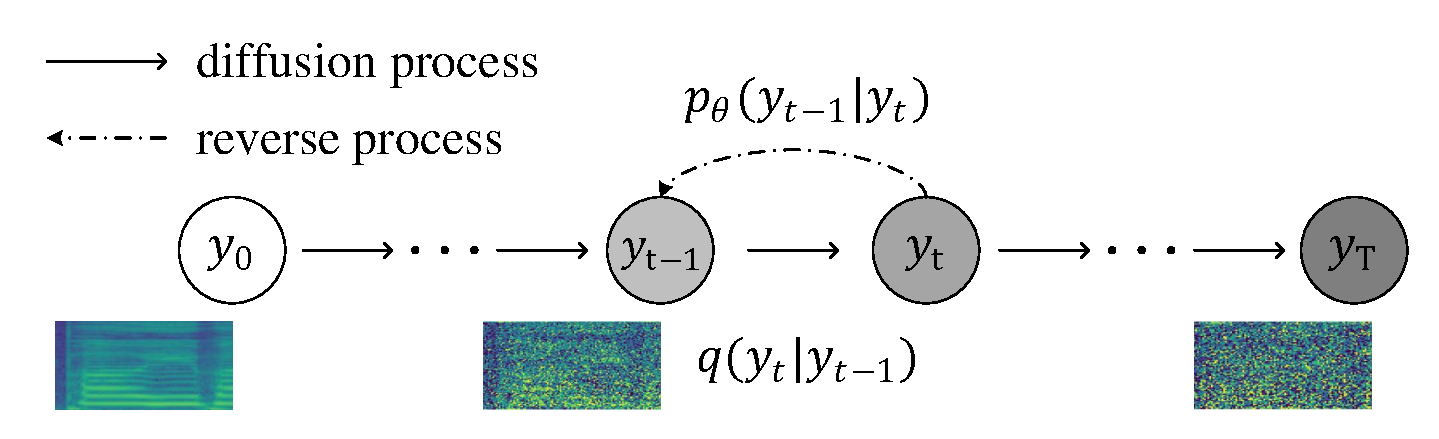
\includegraphics[width=0.99\textwidth]{figure/svs/diffusion-new.pdf}
	\caption{一个简单的扩散模型正向、逆向过程示意图。}
	\label{fig:two_process}
\end{figure}
\subsection{正向扩散过程}
将所要建模的数据的分布定义为$q(\by_0)$,从该分布中进行采样得到$\by_0\sim q(\by_0)$。正向扩散过程本质上是一个相关参数固定的马尔可夫链~\citep{Ho2020ddpm},是将采样得到的$\by_0$在$T$步后变为一个隐变量$\by_T$的过程:
\begin{equation}
  q(\by_{1:T} | \by_0) \defeq \prod_{t=1}^T q(\by_T | \by_{t-1} )
\end{equation}
在$[1, T]$中的每一个扩散时间步$t \in [1, T]$,该过程都会根据一个预先设定好的方差参数的时序变化表$\beta = \{\beta_1, \dotsc, \beta_T\}$来将一个微小的、服从高斯分布的噪声加入上一个时间步的变量$\by_{t-1}$来获得新一个时间步的变量$\by_t$:
\begin{equation}
  q(\by_t|\by_{t-1}) \defeq \mathcal{N}(\by_t;\sqrt{1-\beta_t}\by_{t-1},\beta_t \bI)
\end{equation}
如果方差参数的时序变化表$\beta$设计的合适、总时间步$T$也足够大的话,那么经正向扩散过程最终得到的变量$q(y_T)$的各项都会几乎服从相互独立的高斯分布~\citep{Ho2020ddpm,nichol2021improved}。另外,正向扩散过程还有一个特殊性质,那就是可以在$O(1)$时间内计算出$q(\by_t|\by_0)$这个条件概率分布的封闭形式~\citep{Ho2020ddpm}:
\begin{align}
	q(\by_t|\by_0) = \mathcal{N}(\by_t; \sqrt{\bar\alpha_t}\by_0, (1-\bar\alpha_t)\bI), \label{eq:one_step_noise}
\end{align}
其中,有$\bar\alpha_t \defeq \prod_{s=1}^t \alpha_s$,$\alpha_t \defeq 1-\beta_t$。
\subsection{反向去噪过程}
与正向扩散过程稍有区别的是,反向去噪声过程也是一个马尔可夫链,但是从$\by_T$到$\by_0$的相关参数$\theta$都是可学习的$\theta$。
由于精确的反向过程的转移分布$q(\by_{t-1}|\by_t)$是不可解的,所以需要模型通过具有参数$\theta$(即$\theta$在每个时间步$t$间共享)的神经网络对其进行近似估计:
\begin{equation}
  \label{eq:reverse_step}
  p_\theta(\by_{t-1}|\by_t) \defeq \mathcal{N}(\by_{t-1}; \bmu_\theta(\by_t, t), \sigma_t^2\bI)
\end{equation}
因此,整个反向去噪过程可以按如下方式定义:
\begin{equation}
p_\theta(\by_{0:T}) \defeq p(\by_T)\prod_{t=1}^T p_\theta(\by_{t-1}|\by_t).
\end{equation}
\subsection{训练和采样生成}
为了学习上节定义的模型的参数$\theta$,训练以最小化负对数似然的变分下界的方式进行:
\begin{equation}
\begin{split}
& \mathbb{E}_{q(\by_0)}[-\log p_\theta(\by_0)] \geq \\
& \mathbb{E}_{q(\by_0, \by_1, \ldots, \by_T)}\left[\log q(\by_{1:T} | \by_0) - \log p_\theta(\by_{0:T})\right] \eqqcolon \mathbb{L}.
\end{split}
\end{equation}
对于这一项,公式推导最终得到的结果是用随机梯度下降优化算法针对$\mathbb{L}$中的随机项~\citep{Ho2020ddpm}进行优化:
\begin{align}
\mathbb{L}_{t-1} = \kl{q(\by_{t-1}|\by_t,\by_0)}{p_\theta(\by_{t-1}|\by_t)}, \label{eq:opt_tgtA}
\end{align}
其中,有
\begin{align}
&q(\by_{t-1}|\by_t,\by_0) = \mathcal{N}(\by_{t-1}; \tilde\bmu_t(\by_t, \by_0), \tilde\beta_t \bI)\\
&\tilde\bmu_t(\by_t, \by_0) \defeq \frac{\sqrt{\bar\alpha_{t-1}}\beta_t }{1-\bar\alpha_t}\by_0 + \frac{\sqrt{\alpha_t}(1- \bar\alpha_{t-1})}{1-\bar\alpha_t} \by_t,
\end{align}
其中,又有$\tilde\beta_t \defeq \frac{1-\bar\alpha_{t-1}}{1-\bar\alpha_t}\beta_t$。公式\eqref{eq:opt_tgtA}则等价于:
\begin{align}
  \mathbb{L}_{t-1} - \mathcal{C}
   = \Eb{q}{ \frac{1}{2\sigma_t^2} \|\tilde\bmu_t(\by_t,\by_0) - \bmu_\theta(\by_t, t)\|^2 }, \label{eq:opt_tgtB}
\end{align}
其中,$\mathcal{C}$一项是常数。通过将式\eqref{eq:one_step_noise}进行重参数化为$\by_t(\by_0, \bepsilon) = \sqrt{\bar\alpha_t}\by_0 + \sqrt{1-\bar\alpha_t}\bepsilon$并选择如下的参数化方式:
\begin{equation} \label{eq:mu_parameterization}
    \bmu_\theta(\by_t, t) = \frac{1}{\sqrt{\alpha_t}}\left( \by_t - \frac{\beta_t}{\sqrt{1-\bar\alpha_t}} \bepsilon_\theta(\by_t, t) \right),
\end{equation}
式\eqref{eq:opt_tgtB}就能被化简为:
\begin{align}
    \Eb{\by_0, \bepsilon}{ \frac{\beta_t^2}{2\sigma_t^2 \alpha_t (1-\bar\alpha_t)}  \left\| \bepsilon - \bepsilon_\theta(\sqrt{\bar\alpha_t} \by_0 + \sqrt{1-\bar\alpha_t}\bepsilon, t) \right\|^2}. \label{eq:opt_tgtC}
\end{align}
最终,将$\sigma_t^2$设定为$\tilde\beta_t$,采样出一个$\bepsilon\sim\mathcal{N}(\bzero,\bI)$,$\bepsilon_\theta(\cdot)$就是神经网络的输出结果。
从$p(\by_T) \sim \mathcal{N}(\bzero, \bI)$中采样出$\by_T$并进行相应的反向去噪过程就实现了获取数据分布中样本的目的。
\section{基于扩散模型的翻唱歌声合成声学模型}
本节将详细叙述本章基于扩散模型构建的用于生成梅尔频谱的翻唱歌声合成声学模型,生成的梅尔频谱经声码器处理后即可得到声音波形。
如图~\ref{fig:main_fig}所示,本章提出的声学模型基于扩散模型构建。由于歌声合成任务要求对条件概率分布$p_\theta(M_{0}|x)$进行建模,其中$M$是梅尔频谱图,$x$是对应于$M$的旋律乐谱,因此,$x$会被加入到扩散模型去噪模型中,作为反向去噪过程中的条件来施加影响。本节首先会描述基于扩散模型的原始版本(见节\ref{sec:naive_DiffSinger});然后,本节通过引入一种全新的浅扩散机制来改善模型性能、提高推理效率(见节\ref{sec:shallow_mechanism})使得模型的实际可用性更强;最后,本节会描述相交边界的预测方法,以便模型自适应地找到浅扩散机制中所需的相交边界(见节\ref{sec:boundary_prediction})。
\subsection{基于扩散模型的翻唱歌声合成声学模型基础版本}
\label{sec:naive_diffsinger}
在基础版本的DiffSinger模型中(即图~\ref{fig:main_fig}中不包括虚线框中的部分):在训练过程中(如图~\ref{fig:main_fig_sub1}所示),DiffSinger模型得到梅尔频谱在正向扩散过程中第$t$时间步时的$M_t$,以时间步$t$和音乐旋律$x$为条件,预测式\eqref{eq:opt_tgtC}中的随机噪声项$\bepsilon_\theta(\cdot)$。 在推理过程中(如图~\ref{fig:main_fig_sub2}所示),DiffSinger模型以从
$\mathcal{N}(\bzero, \bI)$分布中采样的高斯白噪声作为梅尔频谱反向去噪过程的起始点,和之前扩散模型相关工作中的做法类似~\citep{Ho2020ddpm,kong2021diffwave}。然后,反向去噪操作会重复迭代进行$T$次来通过两个步骤对过程中间的样本逐渐去噪:1) 通过去噪模型预测中间时间步的噪声项$\bepsilon_\theta(\cdot)$;2) 根据式\eqref{eq:reverse_step}和式\eqref{eq:mu_parameterization}
用预测出的噪声项$\bepsilon_\theta(\cdot)$从此时间步的$M_t$得到前一时间步$M_{t-1}$:
\begin{equation}
    M_{t-1} = \frac{1}{\sqrt{\alpha_t}}\left( M_t - \frac{1-\alpha_t}{\sqrt{1-\bar\alpha_t}} \bepsilon_\theta(M_t, x, t) \right) + \sigma_t \bz,
\end{equation}
其中,当$t>1$时,有$z\sim\mathcal{N}(\bzero, \bI)$,当$t=1$时,则$z=0$。
最终,根据$x$给出的信息作为条件的梅尔频谱$\mathcal{M}$就生成出来了。
\subsection{模型组件概述}
本节将介绍本章搭建的歌声合成模型所使用的各个组件,包括声学模型的参数前端编码器、辅助梅尔频谱解码器,扩散模型的时间步表示嵌入层、去噪模型等。
\subsubsection{声学参数前端编码器}
前端编码器负责将乐谱表达的旋律和歌词编码成歌声的条件序列,所以前端编码器的结构主要包括:1)歌词编码器,用于将歌词文本转化成的音素ID序列映射成嵌入表示序列,以及一系列堆叠的Transformer层~\citep{vaswani2017attention}来将该序列转换为更复杂的隐藏层表示序列;2)长度预测调节器,用于根据旋律中的持续时间信息将隐藏层表示序列以和持续时间相对应的方式扩展到梅尔频谱图的长度;3)音调编码器,用于将离散的MIDI音调ID序列映射成音调嵌入表示序列。最后,前端编码器会按照\citet{ren2020deepsinger}一文中的做法,将文本的隐藏层序列和音调嵌入表示序列加在一起得到旋律条件序列$E_m$。
\subsubsection{辅助梅尔频谱解码器}
本章提出的模型中使用了一种结构简单的解码器作为辅助梅尔频谱解码器,由堆叠前馈Transformer(Feed-Forward Transformer,FFT)层组成,最终输出$\widetilde{M}$,与FastSpeech 2模型~\citep{ren2021fastspeech}中使用的梅尔频谱解码器结构相同。
\begin{figure}[ht]
    \centering
    \subfloat[前端编码器]{
    	\centering
    	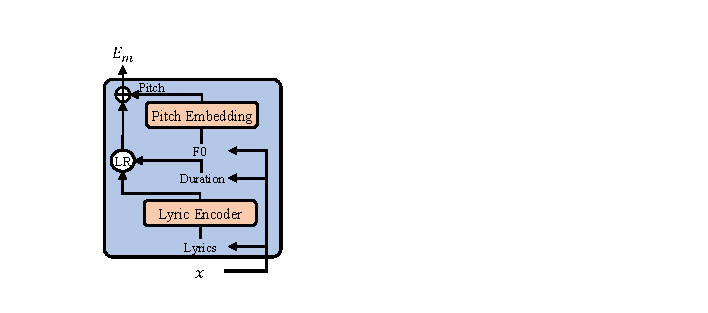
\includegraphics[width=0.45\textwidth,clip=true]{figure/svs/Encoder.pdf}
    	\label{supfig:encoder}
    }
    \subfloat[辅助解码器]{
    	\centering
    	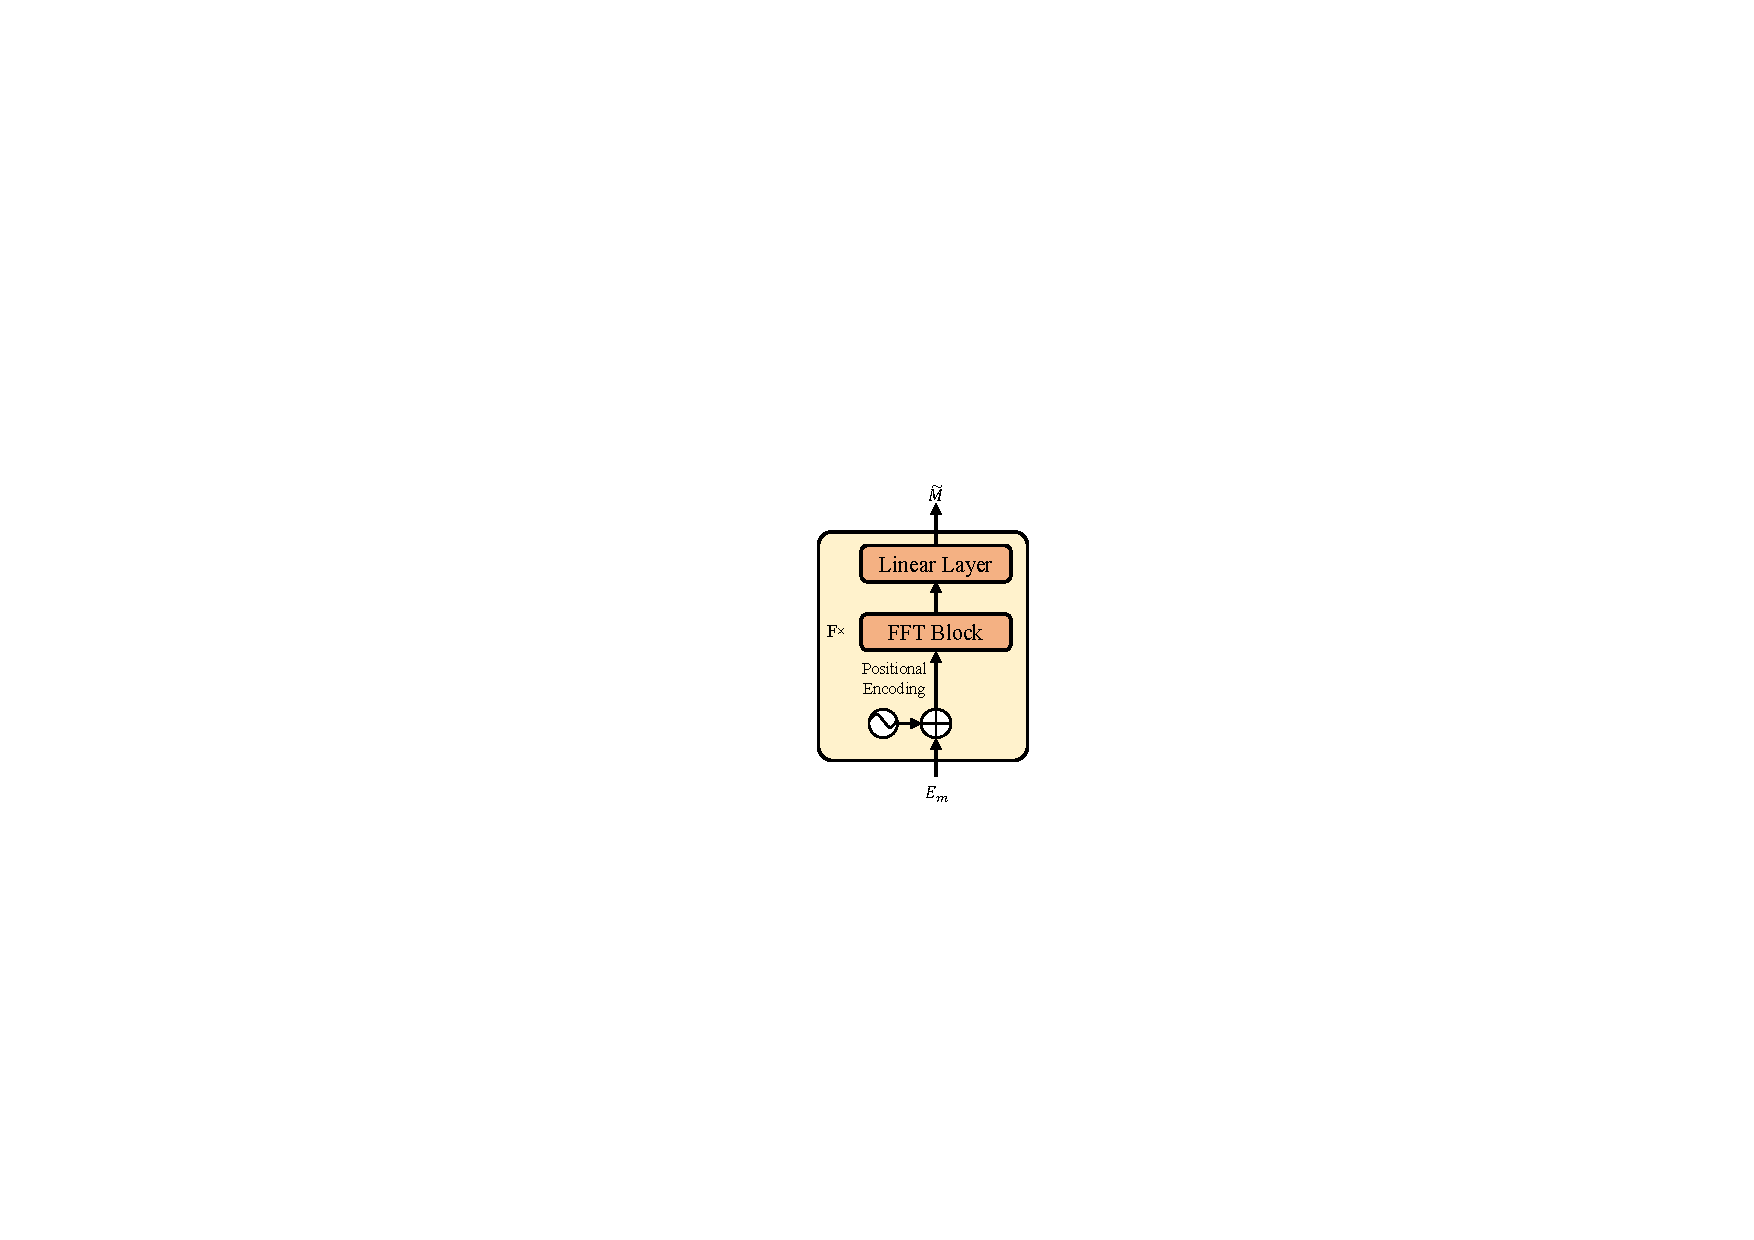
\includegraphics[width=0.45\textwidth,clip=true]{figure/svs/auxiliary_decoder.pdf}
    	\label{supfig:aux_decoder}
    }
    \caption{前端编码器和辅助解码器详细的模型结构图示。$x$表示音乐乐谱信息,$E_m$表示音乐音符所代表的条件序列。 $\widetilde{M}$表示由辅助解码器生成的有模糊现象的梅尔频谱。辅助解码器的训练使用的是L1损失。}
    \label{supfig:encoder_auxdecoder}
\end{figure}
\subsubsection{时间步表示嵌入层}
如上节中式\eqref{eq:opt_tgtC}所述,扩散时间步$t$是去噪模型$\bepsilon_\theta$接受的另一个输入条件。为了将离散的时间步变量$t$变成连续的隐藏层表示,这里的时间步表示嵌入层使用了正弦函数位置嵌入层~\citep{vaswani2017attention},后接两层线性层来得到频道数为$C$的时间步嵌入表示$E_t$。
\subsubsection{去噪模型}
去噪模型$\bepsilon_\theta$以扩散时间步$t$时的中间样本$M_t$为输入,以时间步嵌入表示$E_t$和音乐旋律条件序列$E_m$为条件,来预测正向扩散过程中添加的噪声项$\bepsilon$。由于扩散模型本身并没有对模型架构提出什么约束~\citep{sohl2015deep,kong2021diffwave}, 所以降噪模型的设计其实有很多选择。这里,
本章采用了\citet{rethage2018wavenet,kong2021diffwave}
中提出的非因果式的WaveNet~\citep{vanwavenet}结构作为去噪模型的主干网络。基于WaveNet的去噪模型由一些$1\times1$卷积层组成,可以将$H_m$个信道的梅尔频谱$M_t$映射为有$C$个信道的隐藏层输入表示序列$\mathcal{H}$。之后,还有$N$层堆叠的带有残差连接的卷积层组对隐藏层输入表示序列进行处理。每个卷积层组包括:1)逐分量的加法运算,用于将时间步嵌入表示$E_t$加到$\mathcal{H}$;2)非因果性的卷积网络,用于将$\mathcal{H}$ 从$C$个信道映射出$2C$个信道;3)$1\times1$卷积层,用于将音乐旋律条件序列表示$E_m$映射为$2C$个信道;4)门控单元,用于融合输入的梅尔频谱得到的隐藏层表示序列和其他条件表示;5)残差连接模块,用于将融合后的隐藏层表示平分为各有$C$个信道的两支,即下面的$\mathcal{H}$和将加在最终结果上的``skip hidden''部分,这使得去噪模型能合并使用各个层级的特征表示来给出最终的预测结果。
\begin{figure}[htbp]
	\centering
	\small
	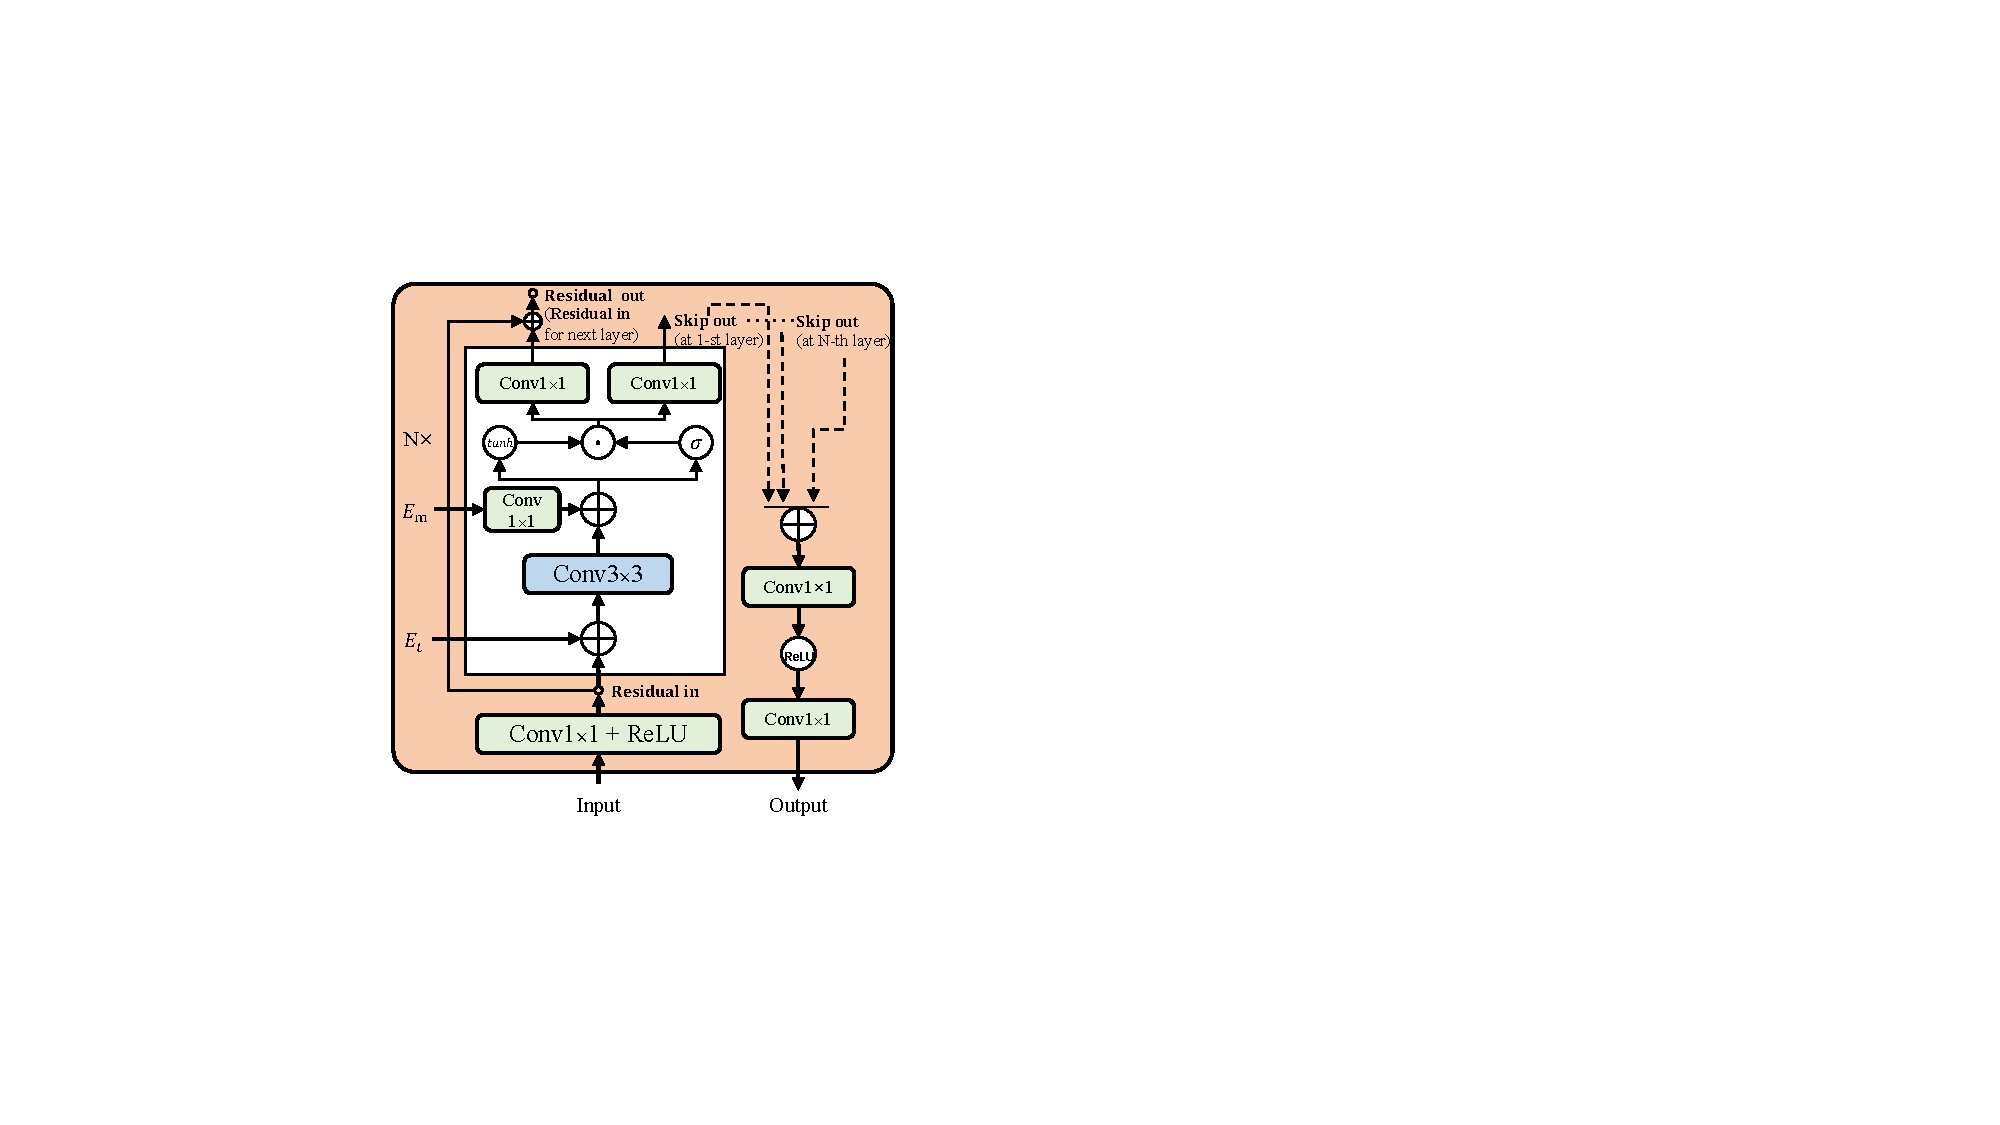
\includegraphics[width=0.99\textwidth,]{figure/svs/denoiser.pdf}
	\caption{去噪模型的详细模型结构图示。$E_t$表示扩散时间步的嵌入表示,$E_m$是音乐旋律条件序列。$N$是残差连接层的层数。去噪模型结构来源于非因果性WaveNet\citep{vanwavenet},但这里因为任务差别将原本设计中的膨胀卷积层替换为普通卷积层做了简化。}
	\label{supfig:denoiser}
\end{figure}
\begin{figure}[ht]
    \centering
    \subfloat[本章提出的基于扩散模型的翻唱歌声合成声学模型训练过程]{
    	\centering
    	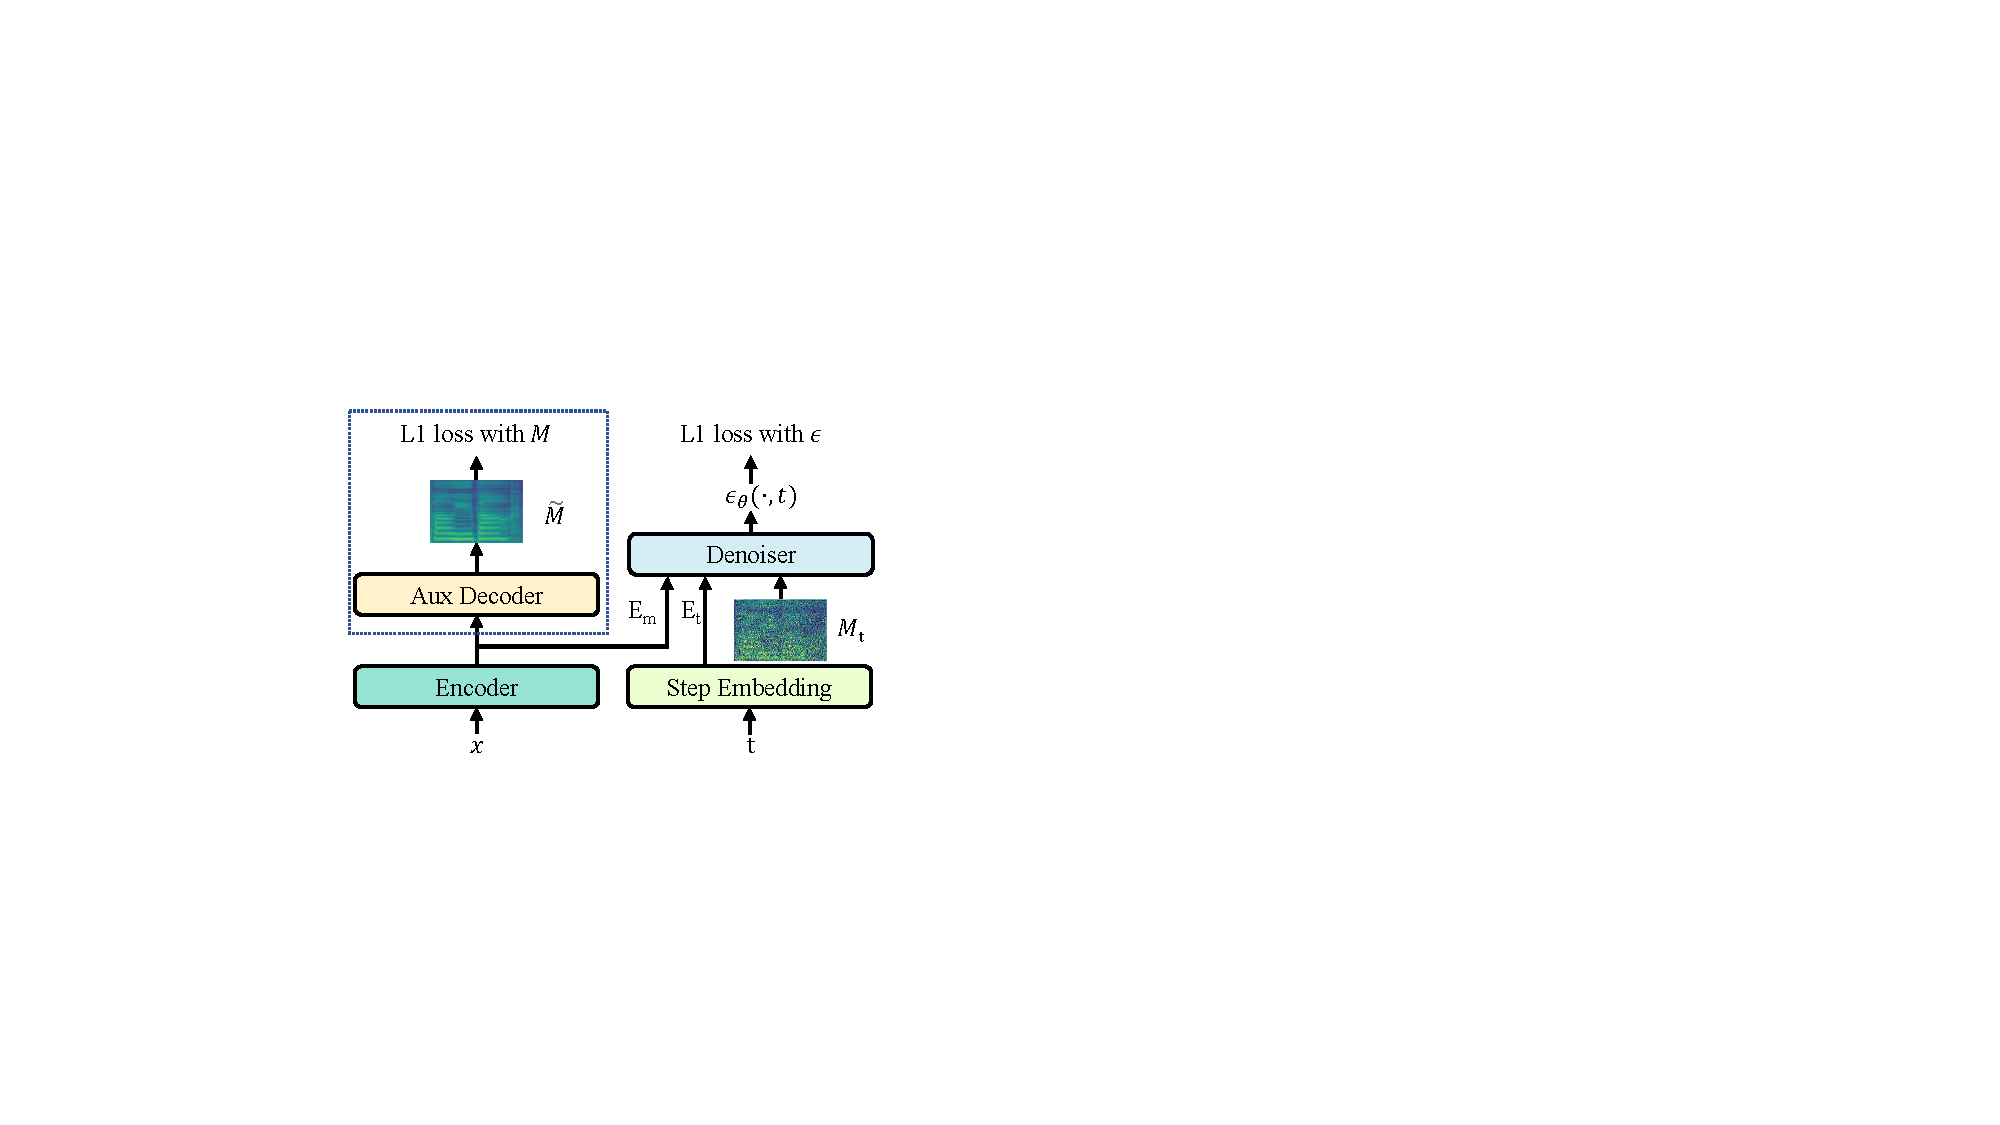
\includegraphics[width=0.99\textwidth,clip=true]{figure/svs/model_a.pdf}
    	\label{fig:main_fig_sub1}
    } \\
    \subfloat[本章提出的基于扩散模型的翻唱歌声合成声学模型的采样推理过程]{
    	\centering
    	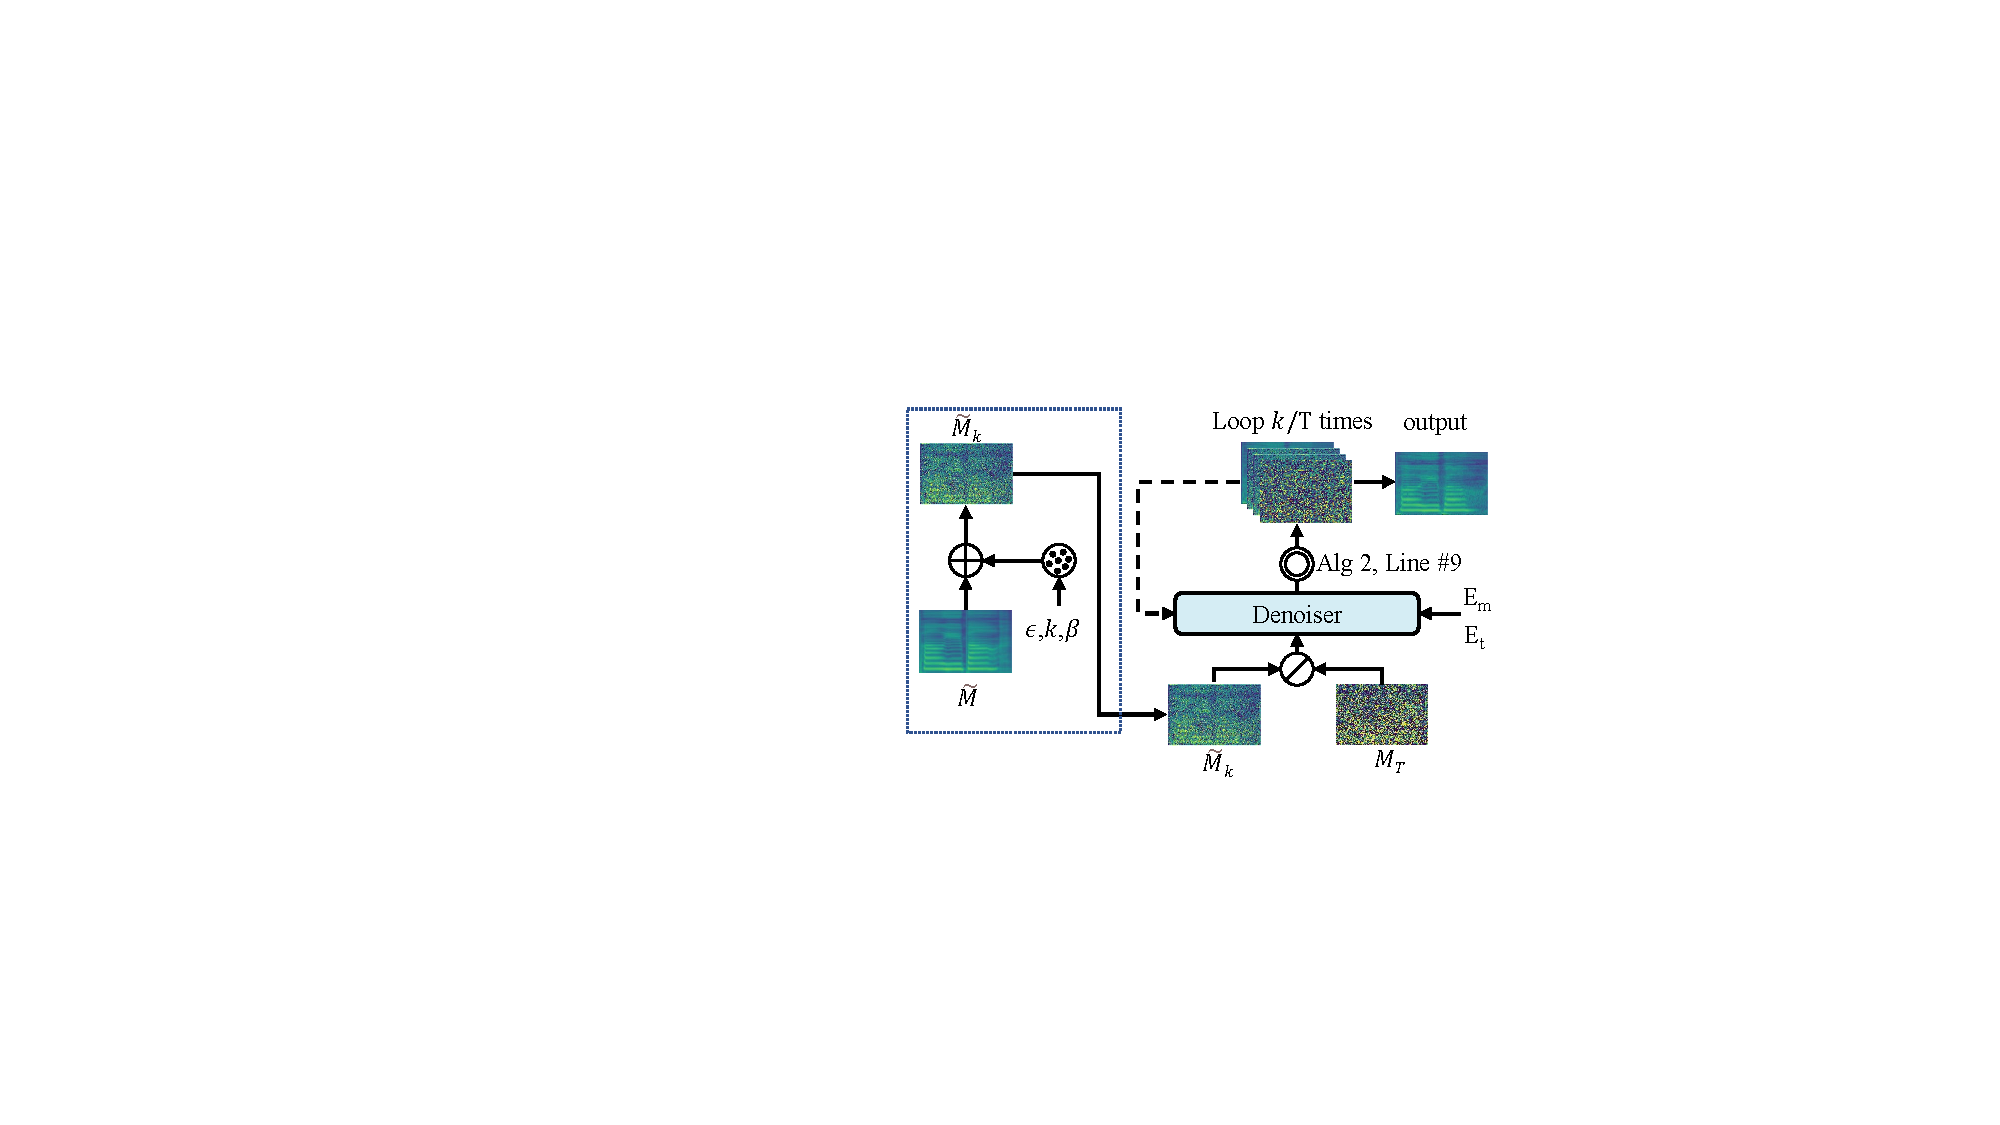
\includegraphics[width=0.99\textwidth,clip=true]{figure/svs/model_b.pdf}
    	\label{fig:main_fig_sub2}
    }
    \caption{本章提出的基于扩散模型的翻唱歌声合成声学模型概览(虚线框中表示模型中的浅扩散机制)。在子图\ref{fig:main_fig_sub1}中,$x$是歌谱信息;$t$是扩散时间步;$M$表示输入的真实波形得到的梅尔频谱;$\widetilde{M}$表示使用L1损失训练出的辅助解码器生成的有模糊现象的梅尔频谱;$M_t$是真实梅尔频谱$M$在正向扩散过程第$t$时间步时的情况。在子图(b)中,$M_T$表示真实梅尔频谱$M$在最大扩散时间步$T$时的情况(接近高斯白噪声);$k$是预测出的浅扩散交汇边界点;开关图标表示可以通过选择使用$M_T$(即基础版本)还是$\widetilde{M}_k$(即浅扩散版本)作为反向去噪过程的起点来控制使用哪个版本的推理过程。}
    \label{fig:main_fig}
\end{figure}
\section{实验设计}
\subsection{歌声合成数据集}
由于本章所涉及的歌声合成研究开始时尚没有公开的高质量中文无伴奏纯歌声数据集,本章收集并标注了一个中国普通话流行歌曲数据集:PopCS,以评估本章提出的模型和方法。PopCS收录了117首中国流行歌曲(总计5.89小时,带有歌词标注),这些歌曲都来自一位专业的女歌手。所有的音频文件都在专业录音室中录制。每首歌曲的音频文件采样率都统一为24kHz,采用16位编码。为了获得与歌曲相对应的更准确的乐谱,本章1)按照DeepSinger~\citep{ren2020deepsinger}一文中的做法,将每首整首歌曲拆分为歌词句的片段,并使用这些句子和音频相对应的片段训练蒙特利尔强制对齐工具(Montreal Forced Aligner,MFA)~\citep{mcauliffe2017montreal}模型,以获得歌曲片段与其对应歌词之间音素级别的对齐;2)使用Parselmouth工具从原始波形中提取$F_0$(基频)作为基音信息,遵循\citet{wu2020adversarially,blaauw2020sequence,ren2020deepsinger}等之前工作中的做法。在实验中,测试集和验证集都是各随机选取了一首歌曲的全部歌曲片段。本章在对这些歌曲进行了清理和分割后,总计得到了1651个歌曲片段,其中大部分片段的持续时间在10-13秒之间。
本章同时使用了一部分歌曲翻译数据集中测试集的数据进行测试。
\subsection{实验设计细节}
为了评估对合成音频质量的直观感受,本章使用了和上一章中类似的平均意见分数(mean opinion score,MOS)和相对平均意见分数(Comparative CMOS)对模型在测试集上的表现进行人工评测。 评测包括了18名合格的听众对合成的歌声和语音音频样本进行判别打分。本章实验会将提出的\textit{DiffSinger}模型生成的歌曲样本和语音样本的人工评测MOS值与以下模型和来源进行比较:1)\textit{GT},真实的音频;2)\textit{GT(Mel + PWG)},此处将真实的歌唱音频先转换为真实的梅尔频谱,然后使用节~\ref{sec:svs_inference}中描述的PWG声码器将这些梅尔频谱转换回音频;3)\textit{FFT-NPSS(WORLD)}~\citep{blaauw2020sequence},基于前馈Transformer层构建的歌声合成系统,生成WORLD声码器使用的特征~\citep{morise2016world}并使用WORLD声码器合成音频;4)\textit{FFT-Singer (Mel + PWG)} 基于前馈Transformer层构建的歌声合成系统,生成梅尔频谱。使用PWG声码器来合成音频;5)\textit{GAN-Singer(Mel + PWG)}
~\citep{wu2020adversarially},使用具有多个随机窗口的鉴别器进行对抗训练的歌声合成系统。
所有模型使用的乐谱旋律条件输入都如前文所述。所有模型使用的都是参数相同的PWG声码器。

另外,为了检验本章提出的模型在语音合成任务上的泛化性能,本节还设计了\textit{DiffSinger}模型在语音合成LJSpeech数据集\cite{ljspeech17}上进行的扩展实验。LJSpeech这个数据集包含13100个英文音频片段(总计约$\sim$24小时)和相应的文本内容。在语音数据集上进行的实验按照FastSpeech 2\citep{ren2021fastspeech}一文中的训练-验证-测试集划分、对梅尔频谱的预处理和音素处理及相应使用的工具\footnote{https://github.com/Kyubyong/g2p}。为了构建本章提出的模型相应的语音合成声学模型\textit{DiffSpeech},需要做出如下调整:1)在\textit{DiffSinger}中加入音调和持续时间预测模块,因为此时不再有给定的旋律信息来指导发声的音高和持续时间,方便期间本节使用了中提出的音调和持续时间预测模块;2)对于在LJSpeech数据集上的浅扩散机制,采用$k=70$作为交汇点时间步。
这样,本章的在语音合成任务上的扩展实验与以下模型和来源进行比较:1)\textit{GT},真实的语音音频;2)\textit{GT(Mel + Hifi-GAN)},此处将真实的歌唱音频先转换为真实的梅尔频谱,然后使用最新工作Hifi-GAN声码器将这些梅尔频谱转换回音频;3)\textit{Tacotron2}~\citep{shen2018natural},经典的自回归式声学模型;4)\textit{BVAE-TTS}\citep{lee2020bidirectional},基于双向变分推断构建的非自回归声学模型;5)\textit{Glow-TTS}\citep{kim2020glow},一种轻量的基于生成归一化流的声学模型;6)FastSpeech 2\citep{ren2021fastspeech},经典的非回归声学模型。
实验的评测实验了Amazon Mechanical Turk平台,规定需要10名评测人员来给出人工评测的平均意见分数。其结果如表~\ref{tab:exp_tts}所示。所有比较的声学模型都使用了最新工作HiFi-GAN~\citep{kong2020hifi}作为转换到音频波形的声码器。
\subsection{浅扩散机制}
\label{sec:shallow_mechanism}
由于扩散模型本身推理需要在反向过程迭代地进行若干步去噪声,搭建的声学模型要得到质量较高的梅尔频谱需要进行100步以上的迭代去噪声操作。因此尽管在前章中提到的使用如L1或L2这样比较简单的损失训练得到的歌声合成声学模型生成的梅尔频谱结果存在一些难以克服的缺陷,但是这些模型的合成结果仍然和真实的梅尔频谱的数据分布有着很强的关联。这些生成的梅尔频谱无法保持很好的非周期参数建模质量,但它们的频谱``轮廓''(即谐波成分)依然和真实梅尔频谱的``轮廓''非常相近。所以这些梅尔频谱实际上可以为基于扩散模型的声学模型提供大量可靠的先验知识。
% 为了进一步探索这种联系并找到更好地利用这些先验知识的方法,
% 本节
如果将正向扩散过程的中间结果可视化进行观察(见图~\ref{fig:fake_real_mels_diffusion})就能发现
% 1)当$t = 0$,
真实的梅尔频谱$M$相邻谐波之间有丰富的细节,这些是决定经声码器合成的音频的自然度的重要因素,而使用L1损失训练的声学模型合成的梅尔频谱$\widetilde{M}$则存在过细节模糊现象,这在前章\ref{sec:svs_intro}中已有详细介绍。因此,在正向扩散过程起始点处,$M$和$\widetilde{M}$存在较大差别,但随着时间步$t$逐渐增大,来自这两个不同起始点的样本随之变得越来越无法区分了。
\begin{figure}[!h]
    \centering
    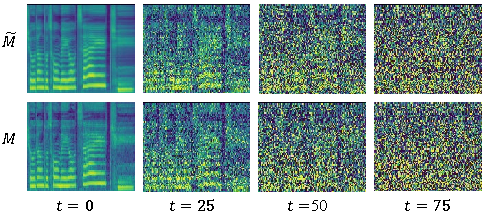
\includegraphics[width=0.99\textwidth,]{figure/svs/fake_real_mel.pdf}
    \caption{正向扩散过程中在各个时间步的梅尔频谱图。第一行展示的是用L1损失训练的辅助解码器生成的梅尔频谱图$\widetilde{M}$的变化情况; 第二行展示的是真实的梅尔频谱图的变化情况。}
    \label{fig:fake_real_mels_diffusion}
\end{figure}
图~\ref{fig:manifolds}中展示的过程说明了这一观察结果的原理性解释:当正向扩散过程走的足够远,即$t$足够大时,当扩散步长足够大时,从$\widetilde{M}$出发进行正向扩散的流形到高斯噪声流形的轨迹和从$M$出发到高斯噪声流形的轨迹会``相交''。
\begin{figure}[ht]
    \centering
    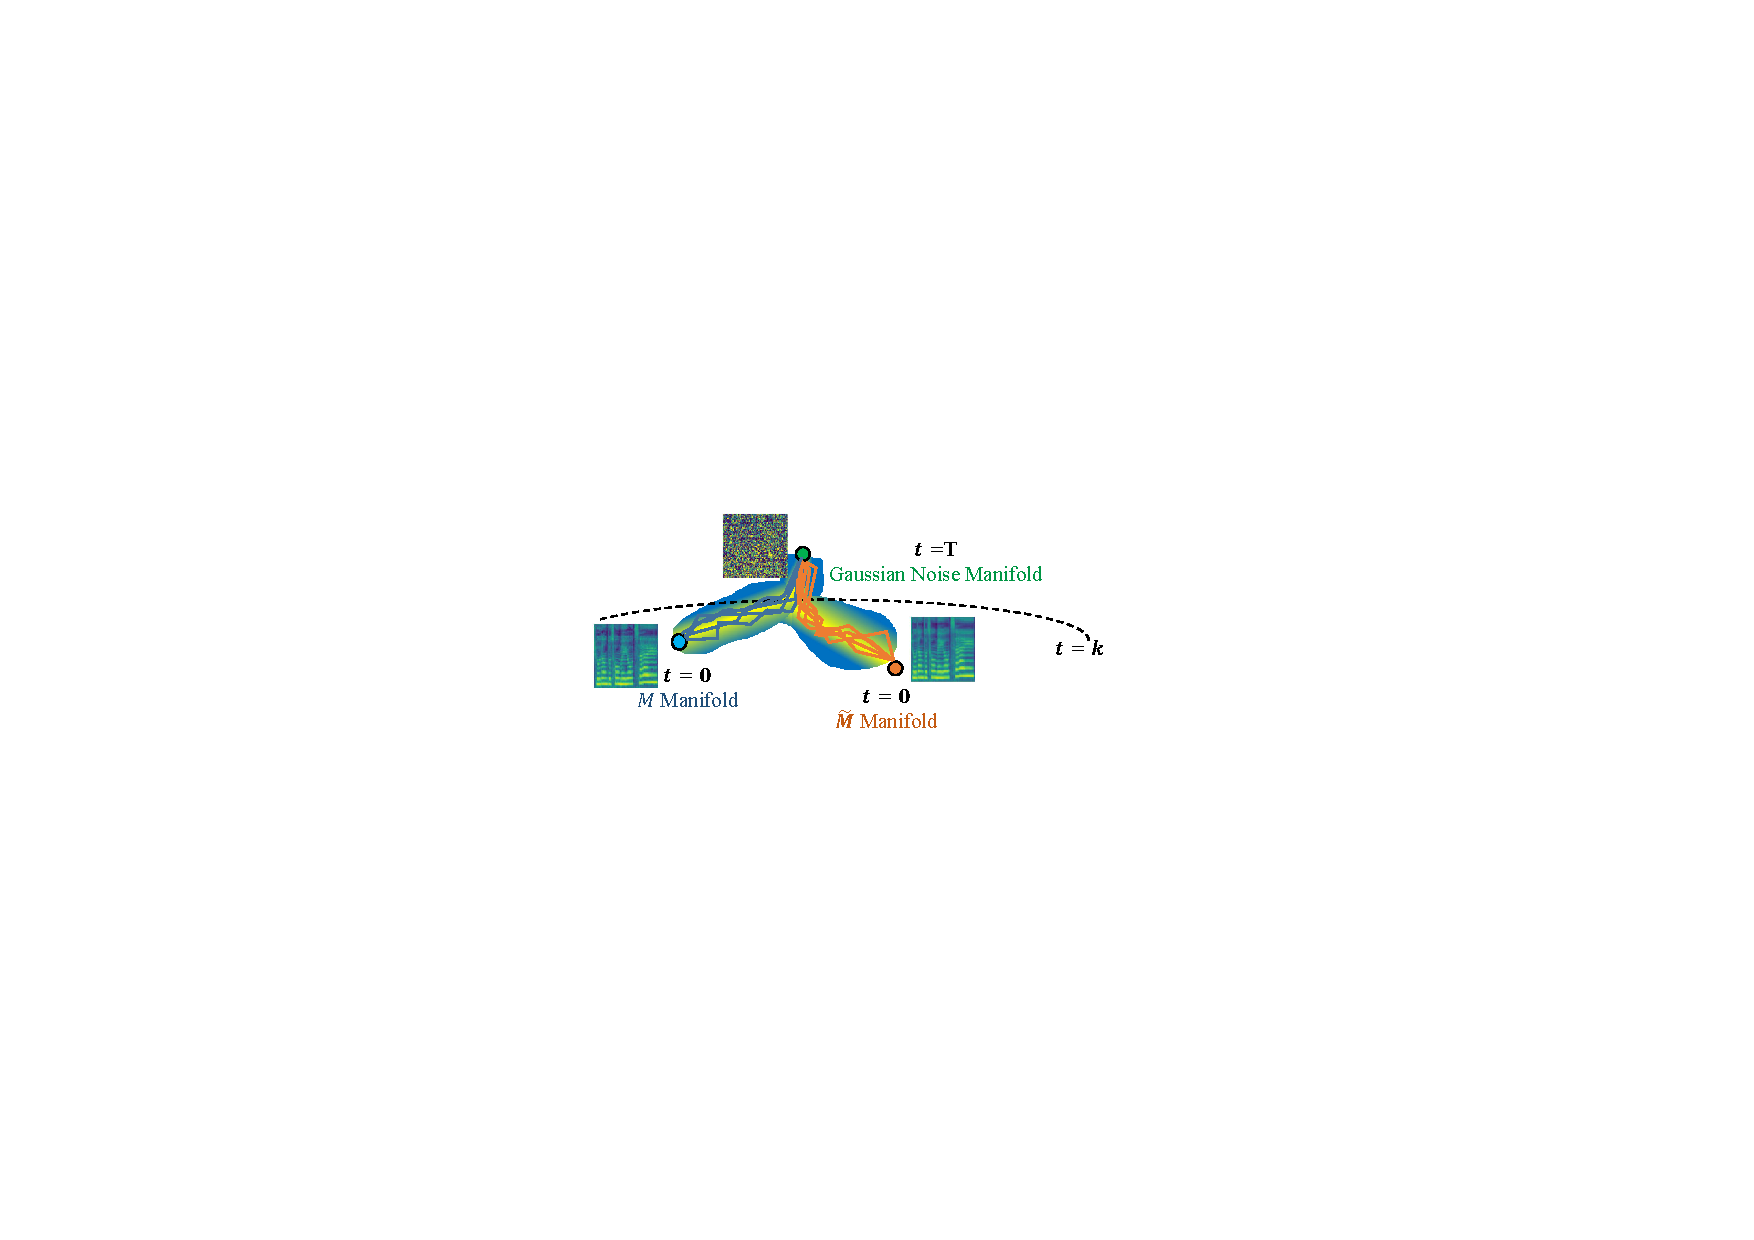
\includegraphics[width=0.99\textwidth]{figure/svs/manifold.pdf} %the ground-truth mel-spectrogram  ; predicted by the simple mel-spectrogram decoder
    \caption{$M$和$\widetilde{M}$在正向扩散过程中的轨迹示意图。$q(M_t| M_0)$和$q(\widetilde{M}_t| \widetilde{M}_0)$这两个分布会随着时间步$t$增大而逐渐接近。}
    \label{fig:manifolds}
\end{figure}
基于这样的观察结果,本节提出了基于扩散模型而进行的浅扩散机制:反向去噪过程不再从高斯白噪声出发,而是从图~\ref{fig:manifolds}中所示的两条轨迹的``交汇点''出发进行。
% 这样,反向去噪过程的负担能获得显著减轻,因为从一个更近的出发点$k$来把$M_k$变换成$M_0$要比从正向扩散过程最远点$M_T$(即高斯白噪声)变换为$M_0$(始终有$k < T$)更容易。因此,前者这种做法就有可能提升模型推理出的梅尔频谱的质量,同时节省从$k$到$T$段反向去噪的变换,因而节省推理时间。
从具体做法上说,使用浅扩散机制和基础版本的基于扩散模型的歌声合成声学模型在推理过程中有这些区别:1) 首先使用一个辅助解码器来生成允许有细节模糊的较低质量梅尔频谱$\widetilde{M}$,这个辅助解码器是使用L1损失函数训练的,同样是以旋律信息的编前端编码器的输出为条件,也就是如图~\ref{fig:main_fig_sub1}中虚线框中所示的部分;
2)如图~\ref{fig:main_fig_sub2}中虚线框中所示,根据式\eqref{eq:one_step_noise}的结论在浅扩散交汇点的时间步$k$通过正向扩散过程得到中间结果:
\begin{equation}
\widetilde{M}_k(\widetilde{M}, \bepsilon) = \sqrt{\bar\alpha_k}\widetilde{M} + \sqrt{1-\bar\alpha_k}\bepsilon,
\end{equation}
其中,有$\bepsilon\sim\mathcal{N}(\bzero, \bI)$,且$\bar\alpha_k \defeq \prod_{s=1}^k \alpha_s$,$\alpha_k \defeq 1-\beta_k$。如果交汇点时间步$k$的选择合适,那么就可以认为$\widetilde{M}_k$和$M_k$是来源于相同的分布的中间样本;
3)以为起始点$\widetilde{M}_k$进行反向去噪过程,即迭代地进行$k$次去噪声操作。
浅扩散机制的训练和推理过程分别在算法~\ref{alg:training}和\ref{alg:sampling}中进行了详细描述。
\begin{algorithm}[!h]
\caption{基于扩散模型的翻唱歌声合成声学模型使用浅扩散机制时的训练过程}
\label{alg:training}
  \SetKwInOut{Input}{Input} %\SetKwInOut{Output}{Output}
    \Input{去噪模型$\bepsilon_\theta$;浅扩散交汇边界点$k$;训练集$(\mathcal{X}, \mathcal{Y})$.}
    % \BlankLine
  \SetKwRepeat{Do}{do}{while}
    \Repeat{收敛}{
        从$(\mathcal{X}, \mathcal{Y})$\;中取数据点$(x, M)$
        $\bepsilon\sim\mathcal{N}(\bzero,\bI)$\;
        $t \sim \mathrm{Uniform}(\{1, \dotsc, k\})$\;
        在\\
        $\quad \grad_\theta \left\| \bepsilon - \bepsilon_\theta(\sqrt{\bar\alpha_t} M + \sqrt{1-\bar\alpha_t}\bepsilon, x, t) \right\|^2$上进行梯度下降优化
     }
\end{algorithm}
\begin{algorithm}[!h]
\caption{DiffSinger模型的推理过程}
\label{alg:sampling}
  \SetKwInOut{Input}{Input} %\SetKwInOut{Output}{Output}
    \Input{去噪模型$\bepsilon_\theta$;辅助解码器;浅扩散交汇边界点$k$;测试集源文本$\mathcal{X}$.}
    % \BlankLine
    从$\mathcal{X}$中采样一个数据点$x$作为条件\;
    用辅助梅尔频谱解码器生成相应的$\widetilde{M}$\;
    $\bepsilon\sim\mathcal{N}(\bzero,\bI)$\;
    $\widetilde{M}_k(\widetilde{M}, \bepsilon) = \sqrt{\bar\alpha_k}\widetilde{M} + \sqrt{1-\bar\alpha_k}\bepsilon$\;
    $M_k =  \widetilde{M}_k$\;
    \For{$t=k, k-1, ..., 1$}{
        \lIf{$t = 1$}{
        $\bz = \bzero$
        }\lElse{采样$\bz \sim \mathcal{N}(\bzero, \bI)$}
        $M_{t-1} = \frac{1}{\sqrt{\alpha_t}}\left( M_t - \frac{1-\alpha_t}{\sqrt{1-\bar\alpha_t}} \bepsilon_\theta(M_t, x, t) \right) + \sigma_t \bz$
     }
\end{algorithm}
% 下一小节将对本节中两条扩散轨迹的交汇等问题给出理论分析和证明。
% \subsection{浅扩散机制的原理和证明}
% \label{sup:proof}
% 本小节将对上一节中的一些结论给出理论分析和证明。
% 给定一个数据分布中的样本$M_0$和相应的辅助解码器生成的结果$\widetilde{M}_0$,那么正向扩散过程中间结果$M_t$和$\widetilde{M}_t$的条件概率分布就分别是:
% \begin{align}
% &q(M_t| M_0)=\mathcal{N}(M_t; \sqrt{\bar\alpha_t}M_0, (1-\bar\alpha_t)\mathbf{I}) \\
% &q(\widetilde{M}_t| \widetilde{M}_0)=\mathcal{N}(\widetilde{M}_t;\sqrt{\bar\alpha_t}\widetilde{M}_0, (1-\bar\alpha_t)\mathbf{I})
% \end{align}
% 这两个正态分布间的KL散度就是:
% \begin{equation}
% \begin{split}
% D_{\mathrm{KL}}\left(\mathcal{N}_{0} \| \mathcal{N}_{1}\right)=\frac{1}{2}[\operatorname{tr}\left(\Sigma_{1}^{-1} \Sigma_{0}\right)+\left(\mu_{1}-\mu_{0}\right)^{\top} \Sigma_{1}^{-1}\left(\mu_{1}-\mu_{0}\right) \\
% -k+\ln (\frac{\operatorname{det} \Sigma_{1}}{\operatorname{det} \Sigma_{0}})]
% \end{split}
% \end{equation}
% 其中,$k$是多维正态分布的维度;$\mu_{0}, \mu_{1}$是先验分布的均值,$\Sigma_{0}, \Sigma_{1}$是协方差矩阵。因此,在本节的这一具体模型中就有:
% \begin{equation}
% D_{KL}(\mathcal{N}(M_t) || \mathcal{N}(\widetilde{M}_t)) = \frac{\bar\alpha_t}{2(1-\bar\alpha_t)} \|\widetilde{M}_0-M_0 \| _2^2
% \end{equation}
% 由于式中的因子$\frac{\bar\alpha_t}{2(1-\bar\alpha_t)}$会随扩散时间步$t$增大而快速减小到0,这个KL散度项整体也会随扩散时间步$t$增大而快速减小到0。这就保证了在正向扩散过程中的这两条扩散轨迹的相交。
%
% 此外,由于辅助梅尔频谱解码器已经通过在训练集上使用简单重建L1损失进行了优化,$\|\widetilde{M}_0-M_0 \| _2^2$也相对被向极小值方向优化了,这更有助于上述证明的轨迹相交结果。另外,交汇点$k$的$\widetilde{M}_k$也不需要与$M_k$完全相同,而只需要来自$q(M_k|M_0)$的附近领域即可,这一点是由梯度得分匹配理论和朗之万动力学的性质所保证的。
% \subsection{浅扩散交汇点的选取}
% \label{sec:boundary_prediction}
本节将继续前一节介绍本章提出的浅扩散机制中交汇点的选取方法。首先,本节提出一种交汇预测器(boundary predictor, BP)来定位图~\ref{fig:manifolds}中显示的交汇点,并相应给出所对应的扩散时间步$k$。具体来说, 交汇预测器由一个按式\eqref{eq:one_step_noise}中的方式向梅尔频谱添加噪声的模块和一个分类器组成。给定过程中某一扩散时间步$t\in[0, T]$,将真实梅尔频谱在该时间步的中间样本$M_t$标记为1类,将辅助梅尔频谱解码器输出的结果在该步的中间样本$\widetilde{M}_t$记为0类,然后使用交叉熵损失来训练交汇预测器中的分类器对输入的在$t$时间步得到的中间样本的梅尔频谱区分是来自真实数据的$M$还是辅助解码器$\widetilde{M}$的。对交汇预测器训练的损失$\mathbb{L}_{BP}$可以写为:
\begin{align*}
    \mathbb{L}_{BP} = - \mathbb{E}_{M\in\mathcal{Y}, t \in [0, T]} [\log BP(M_t, t) + \\
    \log (1-BP(\widetilde{M}_t, t))],
\end{align*}
其中,$\mathcal{Y}$是梅尔频谱训练集。当交汇预测器训练好之后,就可以使用预测器BP的预测值来决定$k$的值,此时BP的预测值就表示样本分类为1,即输入的某时间步下的中间样本来自真实梅尔频谱的概率。对训练集中所有数据样本$ M \in \mathcal{Y}$,
找到一个最小的时间步$k'$使得$[k',t]$中的95\%步骤$t$都满足如下条件:BP($M_t$,$t$)和BP($\widetilde{M}_t$,$t$)之间的差值低于设定的阈值,然后对于所有数据样本求出$k'$的平均值作为轨迹交汇点的时间步$k$。

或者,通过比较KL散度,本节还将提出一种更简单的边界预测的技巧。通过本节前文的叙述可以注意到,交汇点的选取操作可以被视为数据集预处理的步骤之一,相当于对于整个数据集选择一个的超参数$k$。那么,$k$的值实际上可以通过纯暴力搜索整个验证集来手动选择。
凭直觉来说,可以从满足如下条件的所有$t$中选择最小的$t$作为$k$的取值:
\begin{align}
    &\Eb{M\in \mathcal{Y'}}{D_{\mathrm{KL}}\left(\mathcal{N}(M_t)  \| \mathcal{N}(\widetilde{M}_t))\right)} \\
    &=  \Eb{M\in \mathcal{Y'}}{\frac{\bar\alpha_t}{2(1-\bar\alpha_t)} \|\widetilde{M}_0-M_0 \| _2^2}\\ &\leq \Eb{M\in \mathcal{Y'}}{D_{KL}(\mathcal{N}(M_T) || \mathcal{N}(\bzero, \bI))},
\end{align}
上式意味着以时间步$k$的梅尔频谱为反向去噪过程的起始点至少不会比原先使用的先验分布$\mathcal{N}(\bzero, \bI)$作起始点更差。$\mathcal{Y'}$表示验证集中的梅尔频谱图集。此外,当把DiffSinger用在语音合成任务上使用此技巧来确定$k$时,以真实的F0基频和持续时间来生成$\widetilde{M}_t$($\in \mathcal{Y'}$)比使用预测出的量来生成要更合理。
% \subsection{适配浅扩散的模型训练和推理}
\subsection{模型实现和训练细节}
\label{sec:svs_inference}
本章实验通过\textit{pypinyin}工具(\citet{ren2020deepsinger}一文中的做法)将中文歌词转换为音素,训练使用的梅尔频谱都是从真实波形中提取出的,音频使用采样率24kHz,hop size和frame size的大小相应设置为128和512。
文本经处理后的音素词汇表的大小为61。梅尔频谱的bin的数量$H_m$为80。在实际处理中,梅尔频谱的值会被线性缩放到$[-1,1]$范围,基频F0也按照零均值和单位方差进行归一化。
在歌词编码器中,音素嵌入表示的维度为256,Transformer模块的设置与FastSpeech 2~\citep{ren2021fastspeech}中的相同。
在音调编码器中,查找音高表的大小为300,编码的音调嵌入表示的维度为256。前文提到的信道大小$C$也被设置为256。在去噪模型中,卷积层的数量$N$为20,卷积核核大小为3,每个层的膨胀度设置为1(即无膨胀操作),更大的膨胀度可以增加去噪模型的感受野,但经实际实验,这对DiffSinger并无明显作用。
本章实验使用的最大扩散时间步$T$为$100$,噪声规划$\beta$均设置为常数,从$\beta_1=10^{-4}$开始随时间步线性增加到$\beta_T=0.06$。
DiffSinger中使用的辅助解码器的模型设置与FastSpeech 2中使用的梅尔频谱解码器相同。
在交汇点预测器中,卷积层的数量为5,根据实践经验,这里的交汇点预测阈值设置为0.4。


本章提出的DiffSinger模型的训练需要分两个阶段进行:1)预热阶段:用乐谱的前端编码器单独训练辅助解码器约160k步,然后利用辅助解码器的输出训练交汇预测器约30k步,获得交汇时间步$k$的值;2)主要训练阶段:将DiffSinger按照算法~\ref{alg:training}描述的方式训练约160k步,直到收敛。
在推理阶段,对于所有实验,声学模型一致使用预训练过的的ParallelWaveGAN(PWG)~\citep{yamamoto2020parallel}作为声码器,这里由于歌声合成特殊设置,PWG声码器会采用基频F0驱动的激励~\citep{wang2020using}作为附加输入,类似于\citet{chen2020hifisinger}中的做法。然后声码器公平地将声学模型生成的梅尔频谱转换为波形。
\section{实验结果与分析}
主要实验评测结果见表~\ref{tab:main_exp}。真实音频(4.04 $\pm$ 0.11)的平均意见分数应该是声学模型所能生成的音频质量的平均意见分数的上界。本章提出的\textit{DiffSinger}的评测结果大幅优于仅使用如L1或L2的简单训练损失的基线模型 (\textit{FFT-Singer}),与当前最先进的基于对抗训练的模型(\textit{GAN-Singer}~\cite{wu2020adversarially})相比也体现出了相当的优越性,上述结果证明了本章提出的模型和机制的有效性。
\begin{table}[ht]
	\centering
	\caption{95\%置信区间下的歌声样本人工评测的相对意见平均分数结果。``DiffSinger Naive''表示基础版本的DiffSinger模型,没有使用浅扩散机制。}
	\begin{tabular}{l|c}
		\toprule
		Method &  MOS  \\
		\midrule
		\textit{真实音频} & 4.30 $\pm$ 0.09  \\
	    \textit{真实频谱+PWG声码器} & 4.04 $\pm$ 0.11  \\
		\midrule
		\textit{FFT-NPSS+WORLD声码器+} & 1.75  $\pm$ 0.17  \\
		\textit{FFT-Singer+PWG声码器)} & 3.67 $\pm$ 0.11 \\
		\textit{基于对抗训练的声学模型+PWG声码器} & 3.74 $\pm$ 0.12  \\
		\midrule
		\textit{基于扩散模型的声学模型+PWG声码器} & 3.71 $\pm$ 0.10 \\
		\textit{基于扩散模型的声学模型(使用浅扩散机制)+PWG声码器} & \textbf{3.85} $\pm$ 0.11 \\
% 		\textit{DiffSinger$_{large}$ (Mel + PWG)} & 3.75 $\pm$ 0.12 \\
		\bottomrule
	\end{tabular}
	\label{tab:main_exp}
\end{table}
接下来,本节进行了一些消融研究以证明本章提出的模型和方法的有效性,并进行了一些超参数研究以获得最佳模型设置。这些实验都使用了相对意见分数进行人工评估。表~\ref{tab:ablations}中列出了本章提出的基于扩散模型和对抗训练搭建的歌声合成模型的各种变体和不同模型设置的评价结果。从中,可以得出以下几点结论:1)不使用浅扩散机制会导致模型输出的梅尔频谱质量下降(-0.500 CMOS),这与主要实验结果表中的测试结果一致,也验证了本章提出的浅扩散机制的有效性(第一行与第二行结果相比);2)采用其他时间步$k$值(第一行和第三行相比),而不是交汇点预测器预测出的交汇点时间步$k$会导致模型生成的梅尔频谱质量下降,这验证了本章提出的交汇点预测网络可以预测出针对浅扩散机制的合适的时间步$k$;3)信道数为$C=256$且$L=20$的模型输出的结果是表现最佳的(第一行与第二、四、六、七行相比),表明了本章训练时使用的模型设置的参数容量足够得到较好的实验结果。
\begin{table}[ht]
    \small
    \centering
    \caption{95\%置信区间下的歌声样本人工评测的相对意见平均分数结果。在所有实验中,最大扩散时间步$T$的值都为100。$C$是频道数;$L$ 是去噪模型的网络层数; w/ shallow表示``未使用浅扩散机制'';$k=54$是在测试集上得到的浅扩散交汇点。}
    \begin{tabular}[width=\textwidth]{c|c|c|c|c|c}
    \toprule
    No. & $C$ & $L$ & w/ shallow & $k$ & CMOS \\
    \midrule
    1 & 256 & 20  & \checkmark  & 54 & 0.000 \\
    \midrule
    2 & 256 & 20  & $\times$    & -  & -0.500  \\  % 这一行才是真的 ablation study
    \midrule
    3 & 256 & 20  & \checkmark  & 25 & -0.053  \\
    \midrule
    4 & 128 & 20  & \checkmark  & 54 & -0.071  \\
    5 & 512 & 20  & \checkmark  & 54 & -0.044  \\
    \midrule
    6 & 256 & 10  & \checkmark  & 54 & -0.293  \\
    7 & 256 & 30  & \checkmark  & 54 & -0.445  \\
    \bottomrule
    \end{tabular}
    \label{tab:ablations}
\end{table}
接下来,本节针对一些具体示例进行对各个模型合成梅尔频谱优劣的具体分析。
如图~\ref{fig:case_study}所示,将对相同的音乐旋律条件的来自真实音频提取出的梅尔频谱、本章提出的\textit{Diffsinger},基于对抗训练的\textit{GAN-singer}和使用简单训练损失的\textit{FFT-Singer}模型合成的梅尔频谱进行比较。通过比较可以看出,图~\ref{fig:case_fsadv}和图~\ref{fig:case_diff}谐波间的频谱细节要比图~\ref{fig:case_fs2}更细致丰富。
此外,本章提出的\textit{Diffsinger}在中低频区域的性能比\textit{GAN-singer}显得更有竞争力,高频区域的细节质量则差不多。
\begin{figure}[h]
    \centering
    \subfloat[\textit{GT}]{
    	\centering
    	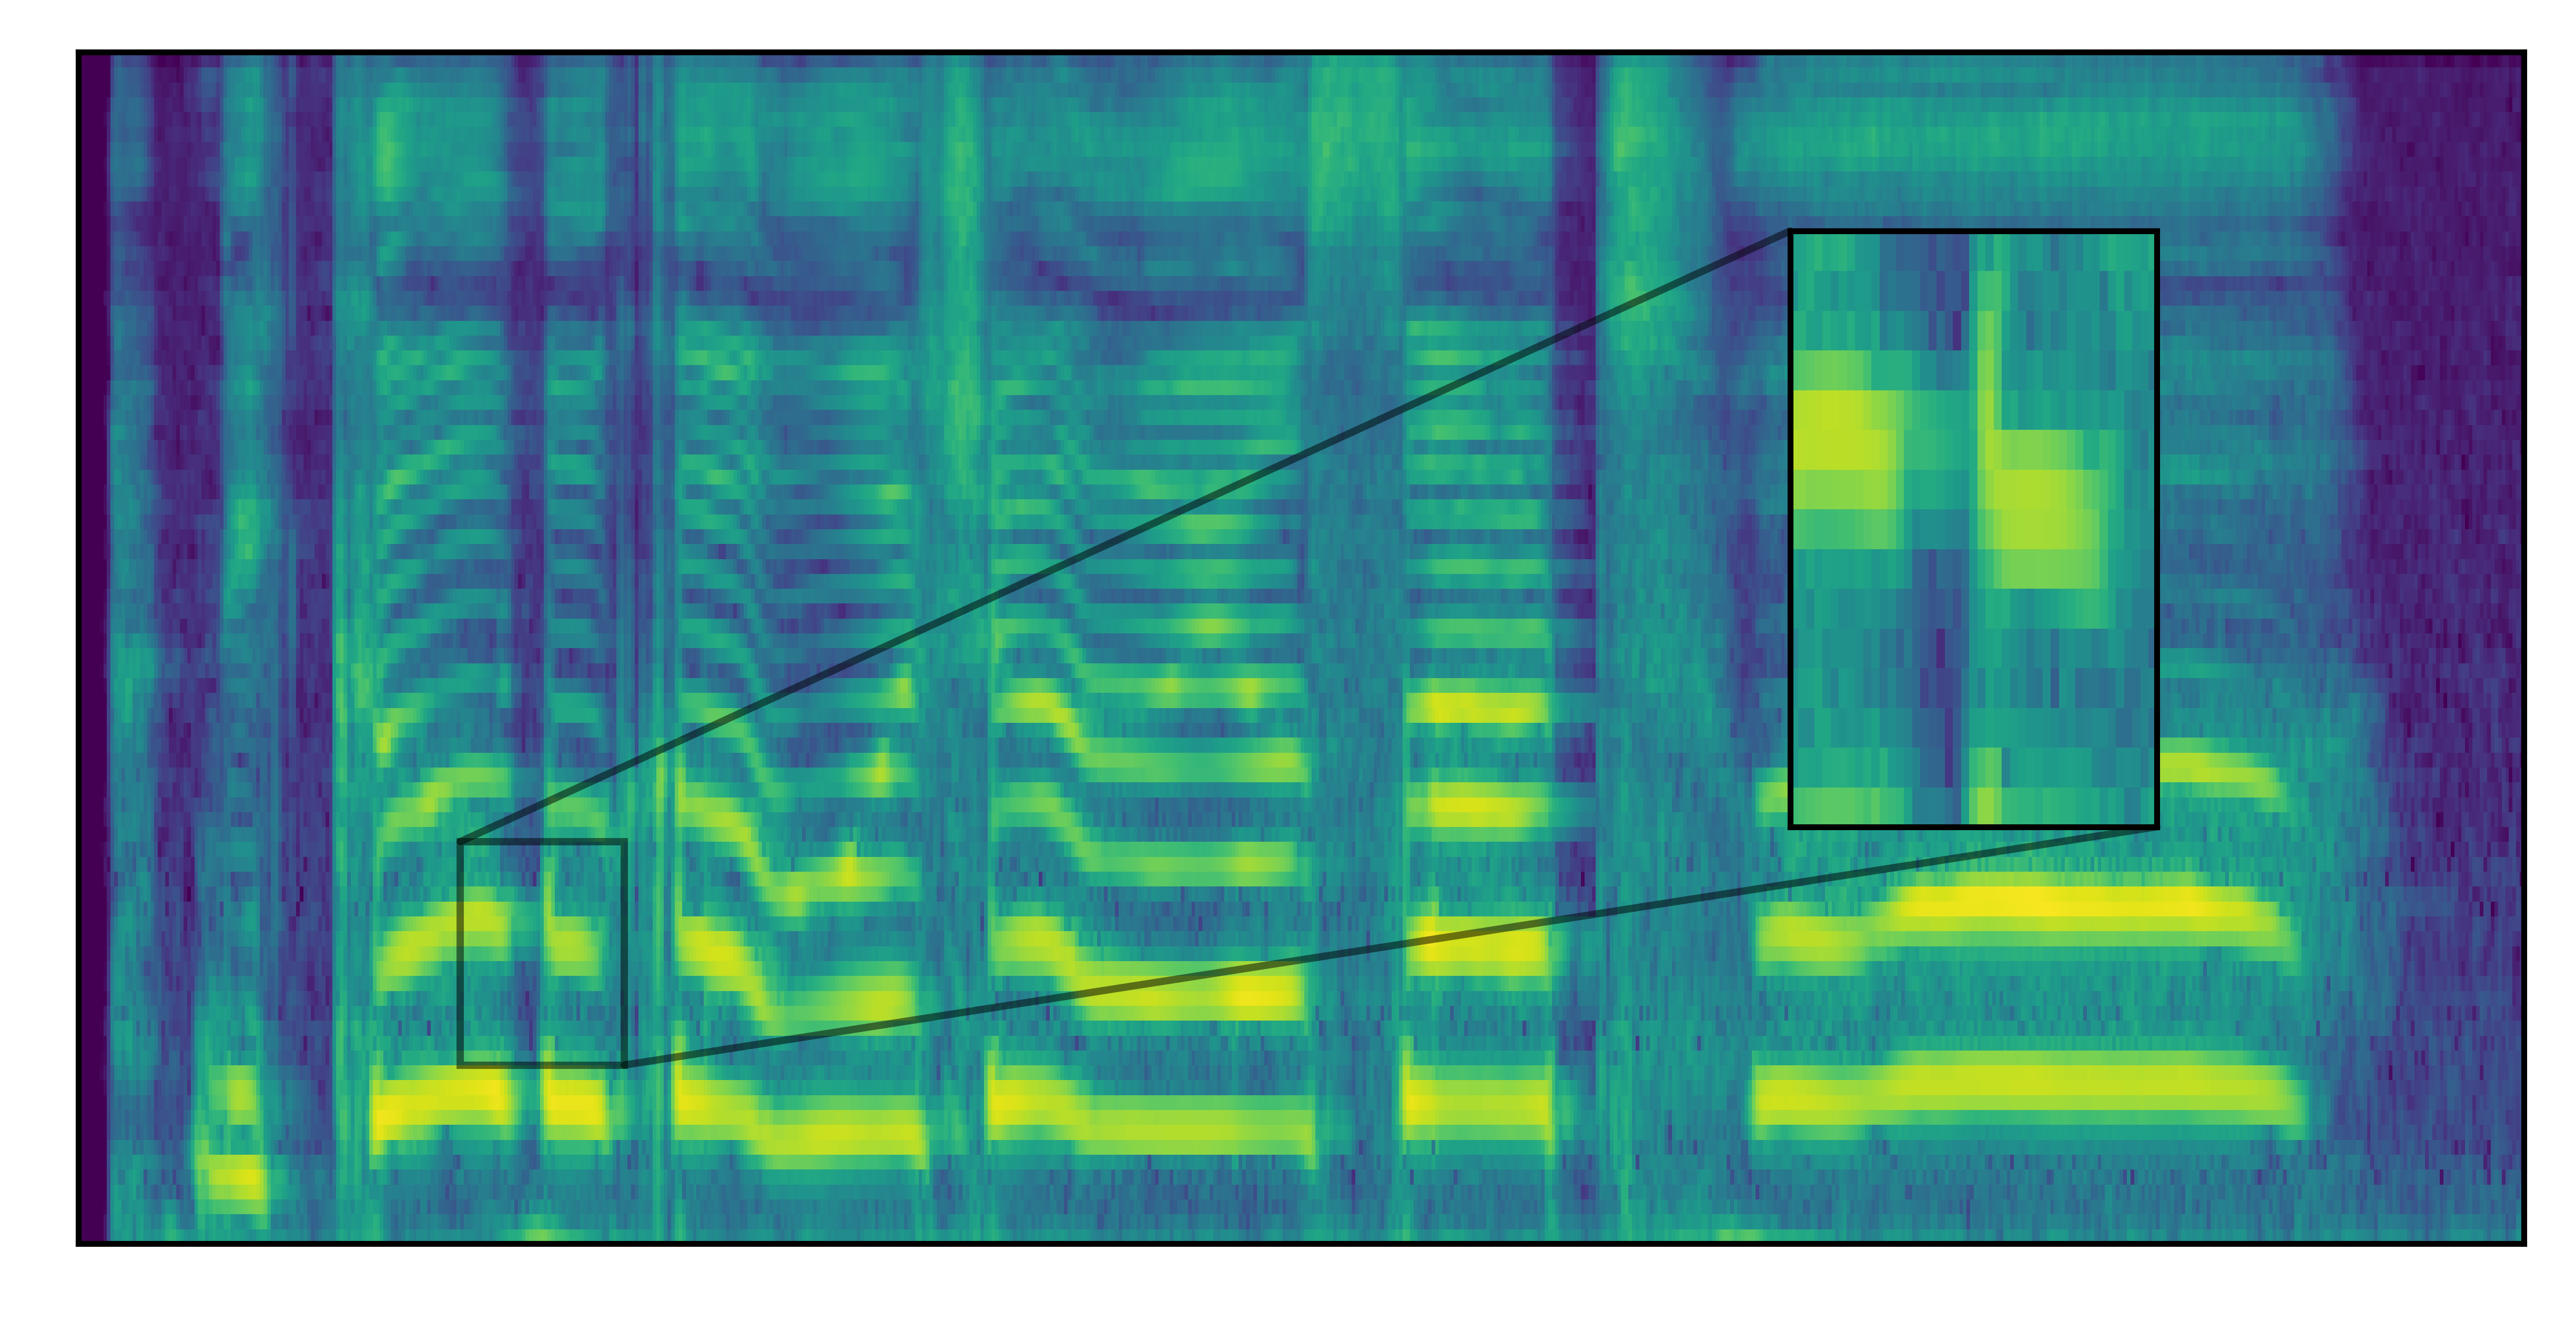
\includegraphics[width=0.49\textwidth,clip=true]{figure/svs/case_GT.png}
    	\label{fig:case_gt}
    }
    \subfloat[\textit{DiffSinger}]{
    	\centering
    	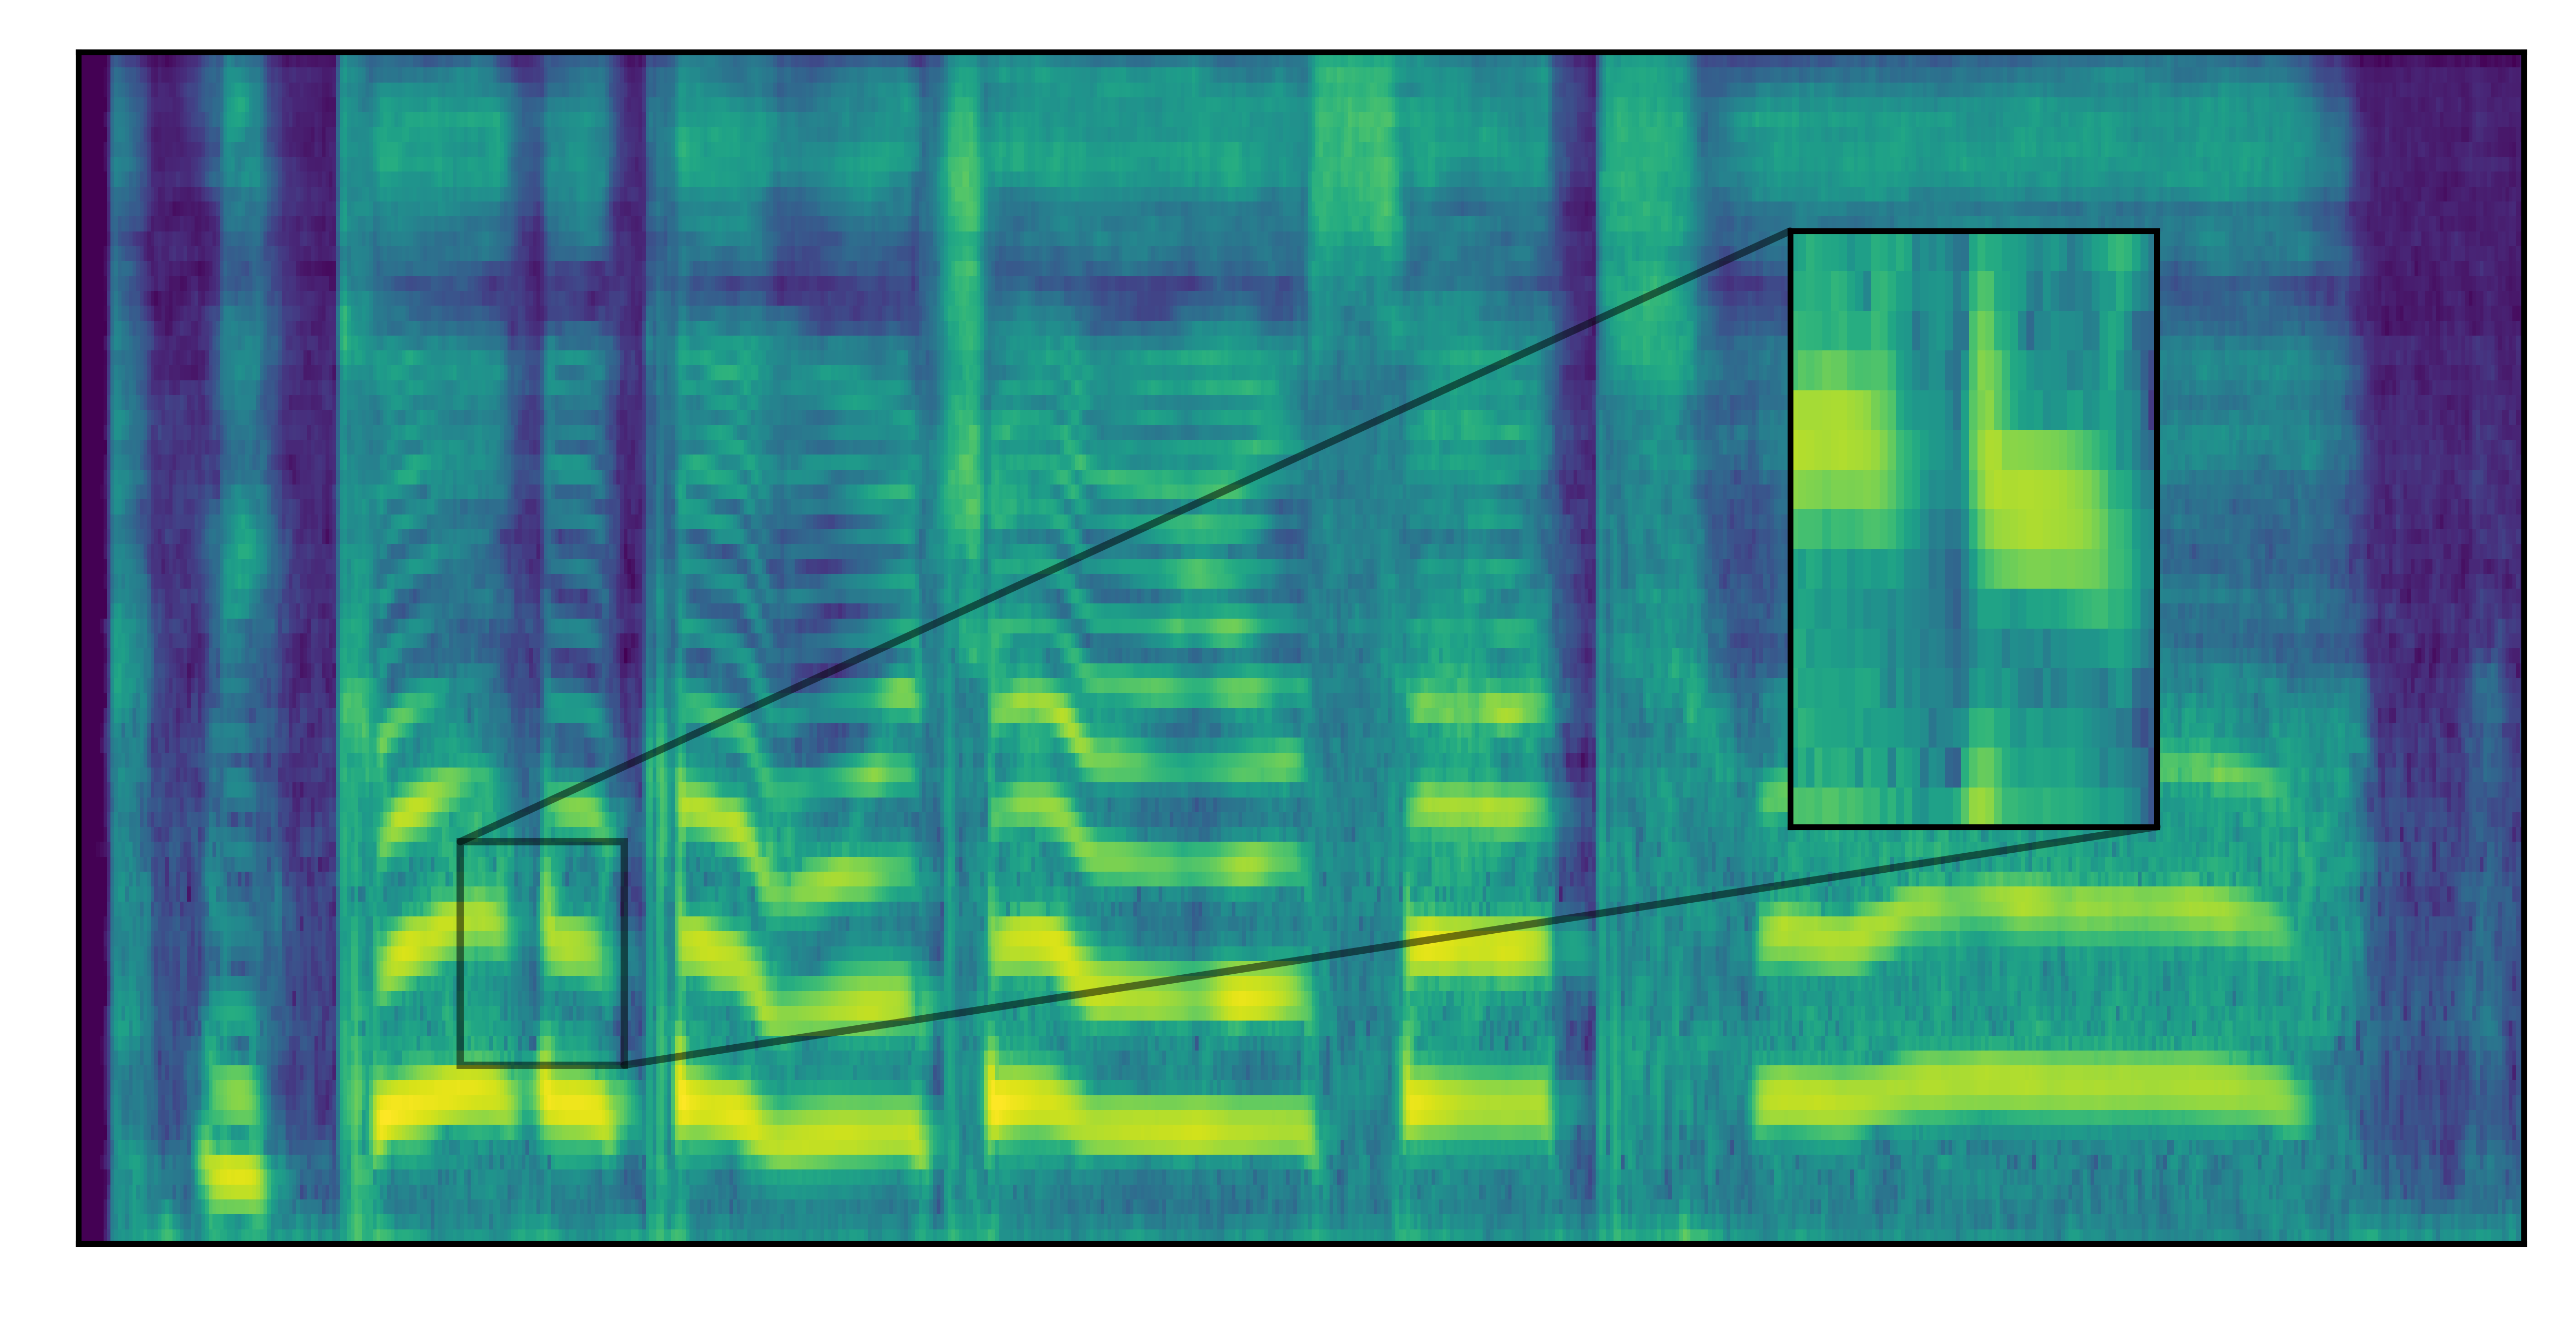
\includegraphics[width=0.49\textwidth,clip=true]{figure/svs/case_diffmel.png}
    	\label{fig:case_diff}
              } \\
    \subfloat[\textit{GAN-singer}]{
    	\centering
    	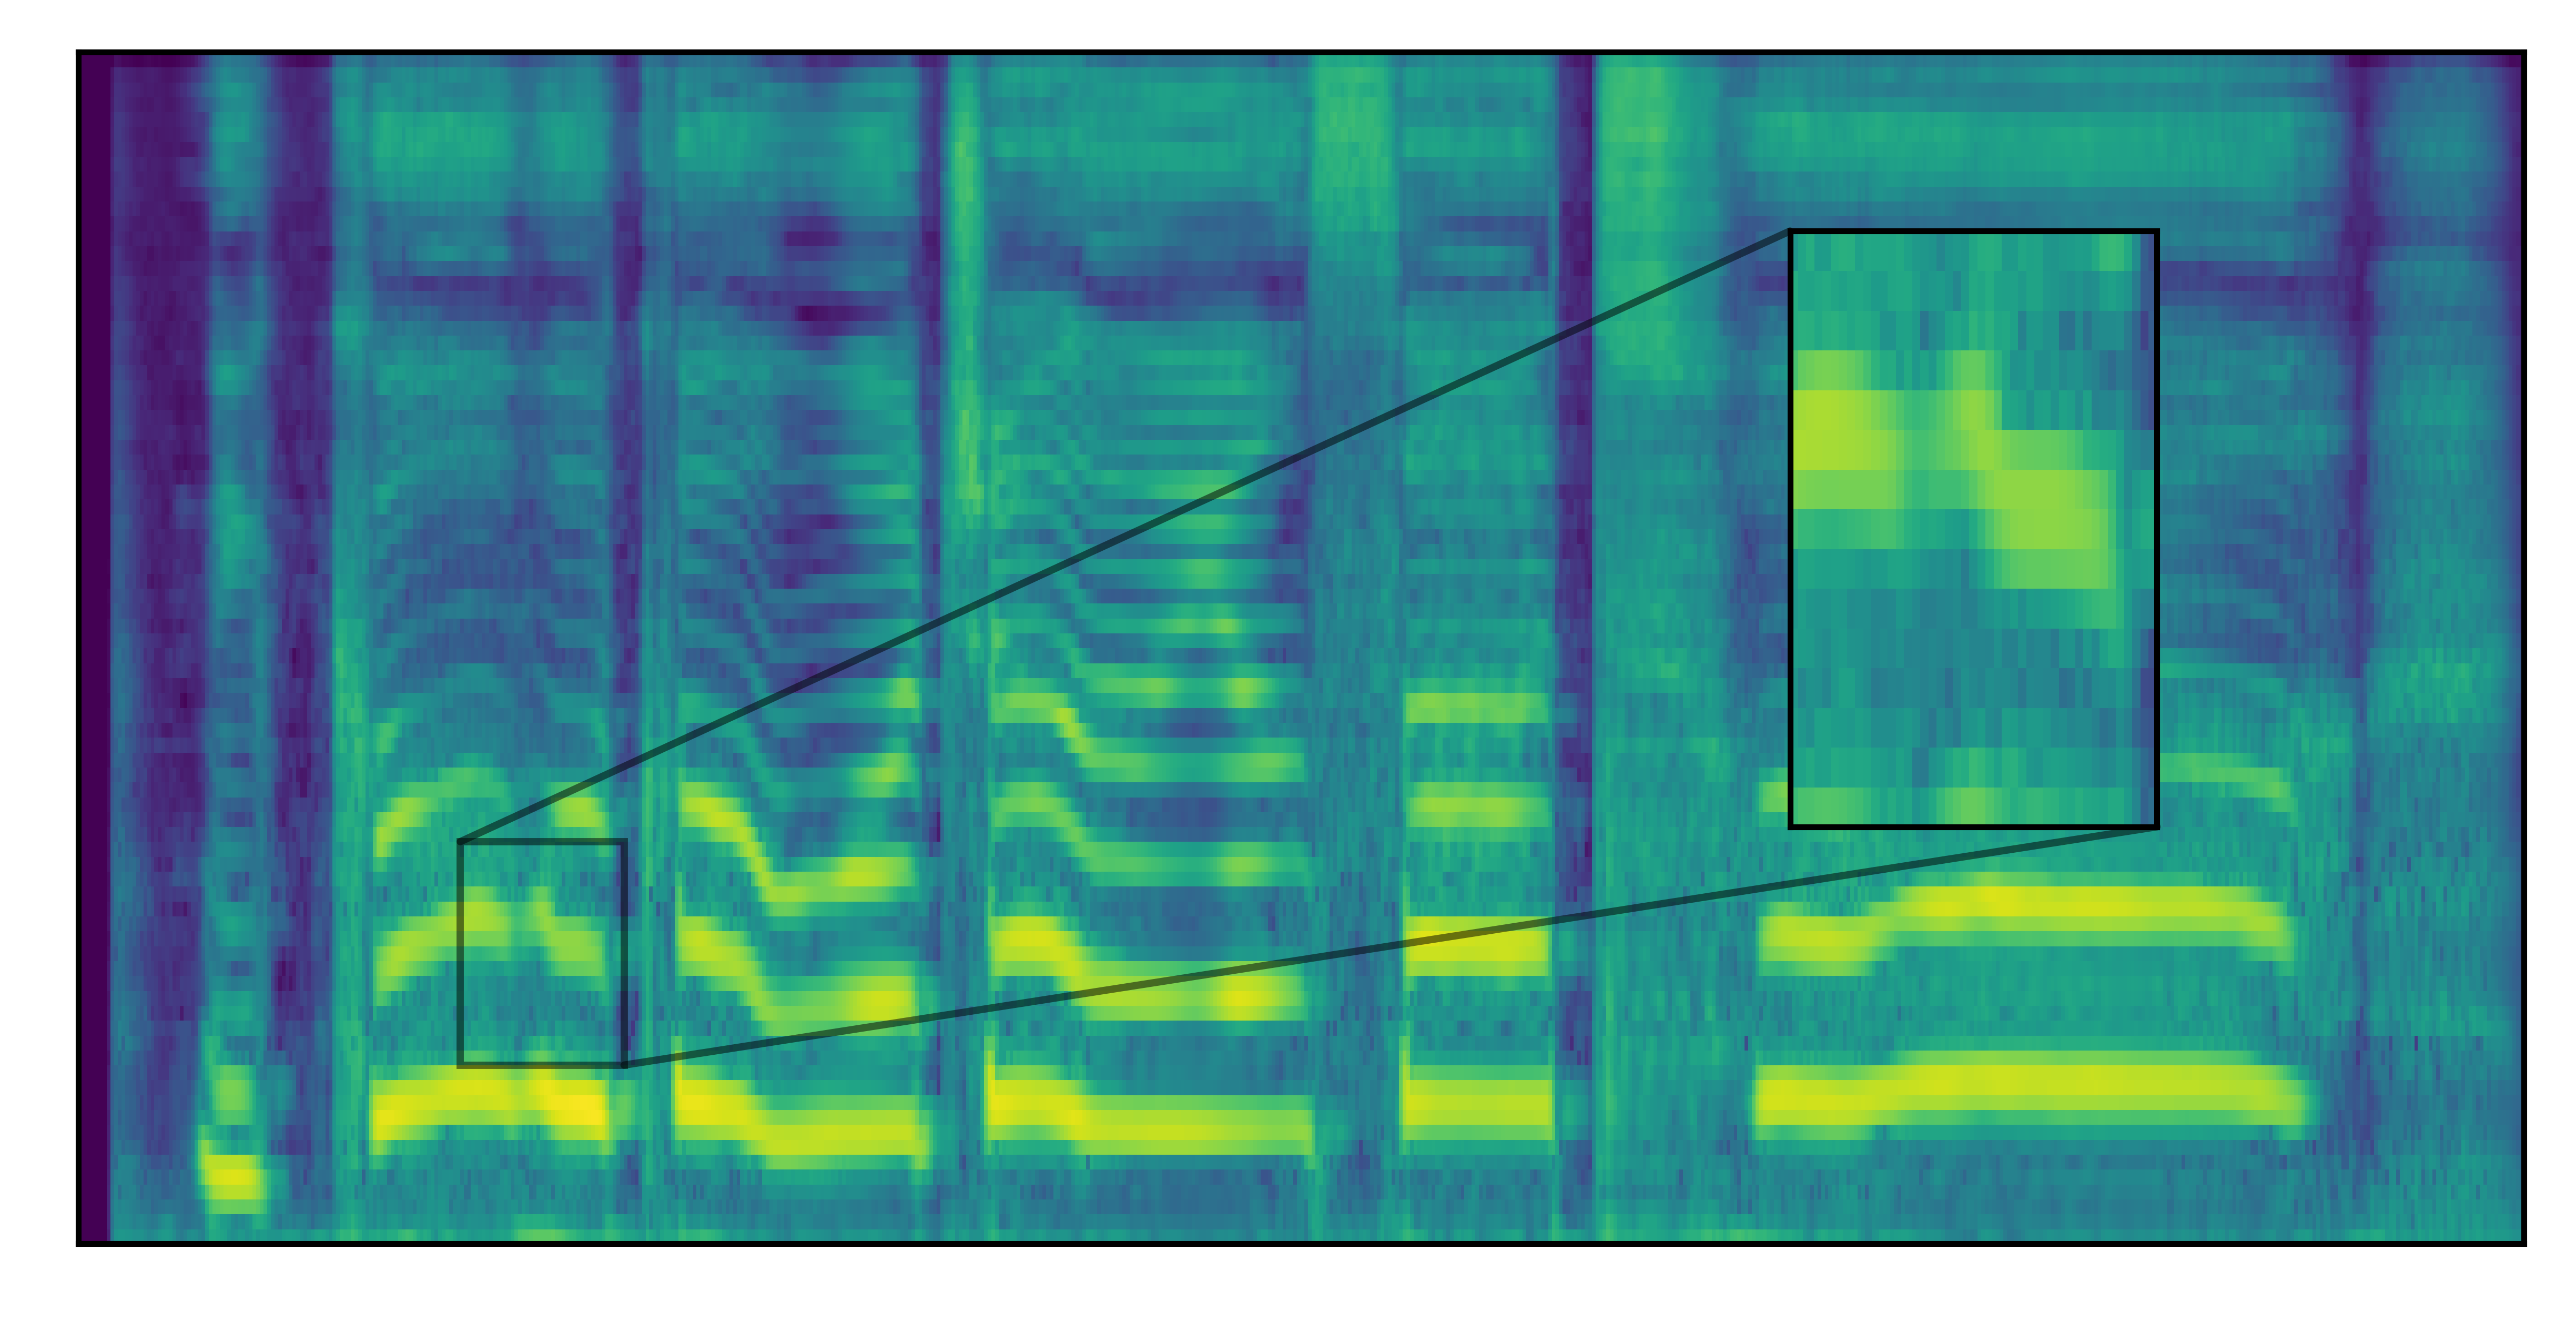
\includegraphics[width=0.49\textwidth,clip=true]{figure/svs/case_fsadv.png}
    	\label{fig:case_fsadv}
             }
    \subfloat[\textit{FFT-Singer}]{
    	\centering
    	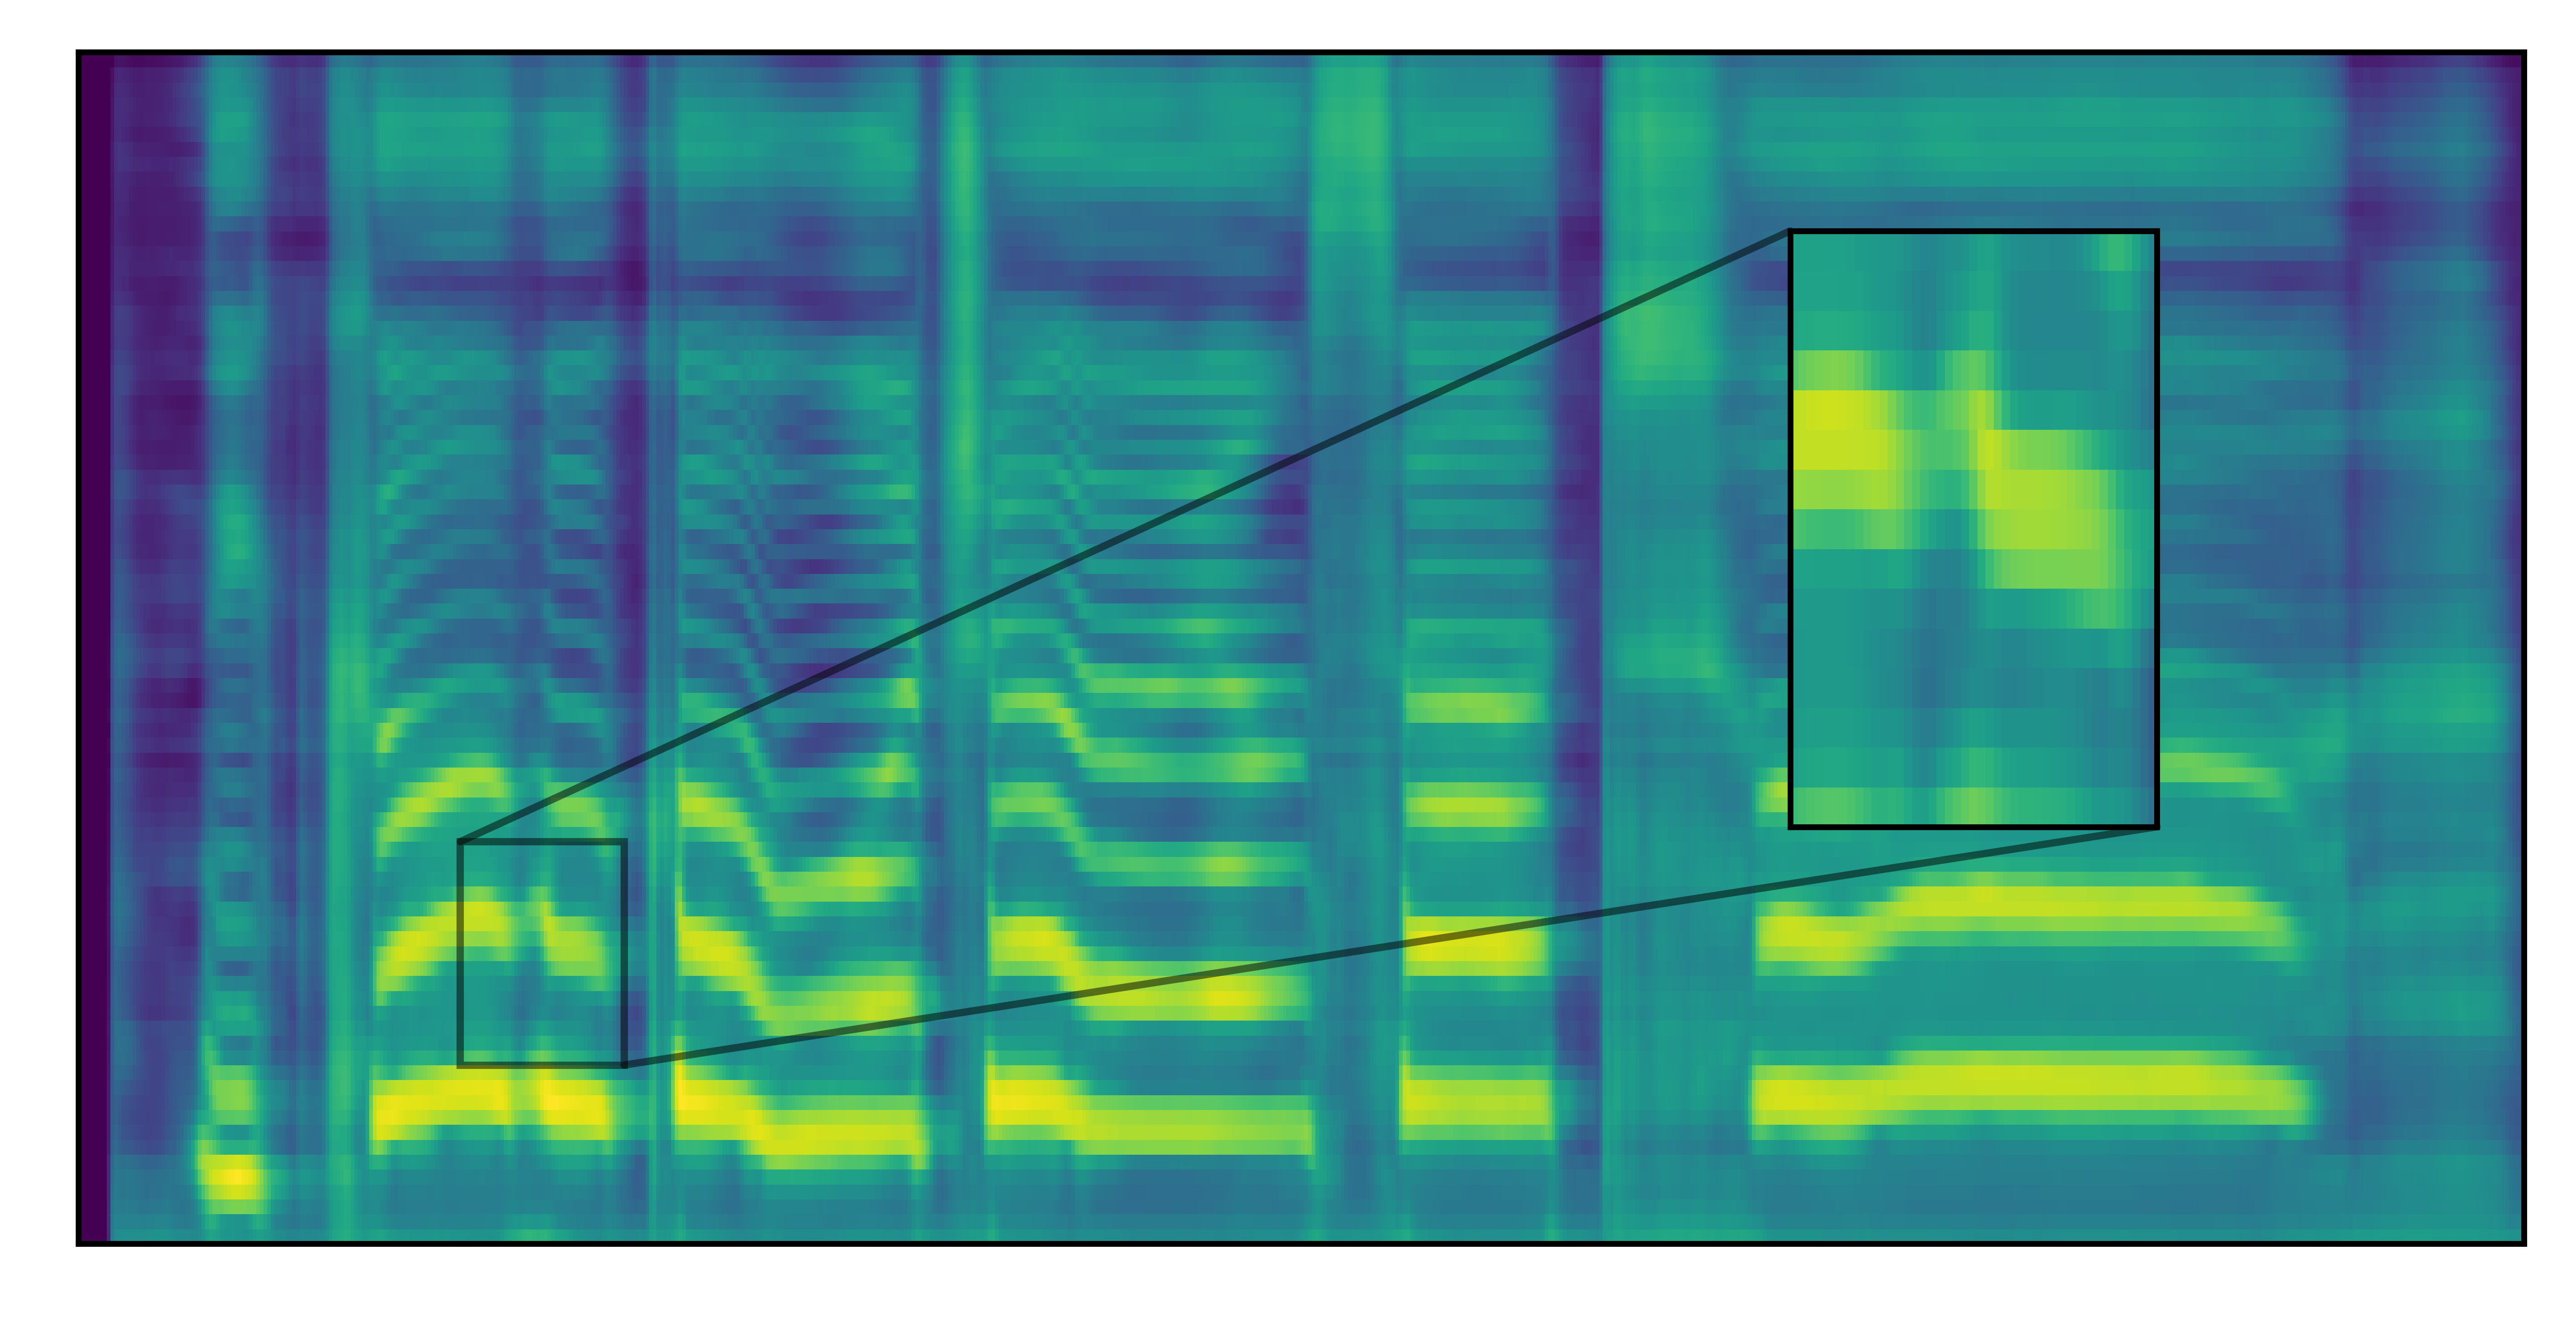
\includegraphics[width=0.49\textwidth,clip=true]{figure/svs/case_fs2.png}
    	\label{fig:case_fs2}
    }
    \caption{来自基于扩散模型的声学模型,基于对抗训练的声学模型和FFT-Singer的梅尔频谱预测结果和真实的梅尔频谱的可视化图。}
    \label{fig:case_study}
\end{figure}
同时,浅扩散机制将原始扩散模型的推理速度加快了45.1\%,以实时因数(RealTime Factor),即生成1秒音频所需的秒数进行衡量,使用浅扩散机制前后的RTF结果分别为0.191 vs.0.348。
表~\ref{suptab:model_size}中汇总了本章实验中进行比较的几个模型的参数量规模。可以看出本章提出的基于扩散模型的翻唱歌声合成模型的可学习参数的规模与其他最先进的模型相比相差无几。
% \begin{table}[h]
%     \centering
%     \begin{tabular}{ l | c }
%     \toprule
%     Method &  MOS \\
%     \midrule
%     \textit{GT} & 4.22 $\pm$ 0.07 \\
%     \textit{GT (Mel + HiFi-GAN)} & 4.15 $\pm$ 0.07 \\
%     \midrule
%     \textit{Tacotron 2 (Mel + HiFi-GAN)} & 3.54  $\pm$ 0.05  \\
%     \textit{BVAE-TTS (Mel + HiFi-GAN)} & 3.48 $\pm$ 0.06 \\
%     \textit{FastSpeech 2 (Mel + HiFi-GAN)} & 3.68 $\pm$ 0.06 \\
%     \textit{Glow-TTS (Mel + HiFi-GAN)} & 3.69 $\pm$ 0.07 \\
%     \midrule
%     \textit{DiffSpeech Naive (Mel + HiFi-GAN)} & 3.69 $\pm$ 0.05 \\
%     \textit{DiffSpeech (Mel + HiFi-GAN)} & \textbf{3.92} $\pm$ 0.06 \\
%     \bottomrule
%     \end{tabular}
%     \caption{95\%置信区间下的语音样本人工评测的意见平均分数结果。}
%     \label{tab:exp_tts}
% \end{table}
\begin{table}[htbp]
\begin{center}
% \small
		\caption{模型的参数量规模比较统计表。}
    \begin{tabular}{ l | c }
        \toprule
        \textbf{模型名称} &  \textbf{参数量(百万)} \cr
        \midrule
        \multicolumn{1}{l}{\textit{SVS Models}}         \\
        \midrule
        DiffSinger & 26.744 \cr
        \midrule
        FFT-Singer & 24.254 \cr
        \midrule
        \multirow{2}*{GAN-Singer}
         ~ & 24.254 (Generator)  \cr
         ~ & 0.963 (Discriminator)  \cr
        \midrule
        \multicolumn{1}{l}{\textit{TTS Models}}         \\
        \midrule
        DiffSinger & 27.722 \cr
        \midrule
        Tacotron 2 & 28.193 \cr
        \midrule
        BVAE-TTS & 15.991 \cr
        \midrule
        FastSpeech 2 & 24.179 \cr
        \midrule
        Glow-TTS & 28.589 \cr
        \midrule
    \end{tabular}
\end{center}

\label{suptab:model_size}
\end{table}
% 另外,为了检验本章提出的模型在语音合成任务上的泛化性能,本节如前文所述,报告模型在LJSpeech数据集\cite{ljspeech17}上进行的扩展实验的结果。语音合成任务人工评测的结果如表~\ref{tab:exp_tts}所示。所有实验中进行比较的声学模型都使用了最新工作HiFi-GAN~\citep{kong2020hifi}作为转换到音频波形的声码器。
% 从表中的实验结果可以看出,\textit{DiffSpeech}的表现也优于FastSpeech 2和Glow TTS,这证明了本章提出的模型和方法良好的泛化性能。此外,表~\ref{tab:exp_tts}中的最后两行的结果同样佐证了浅扩散机制的有效性,加速率为29.2\%,实时因数分别为0.121 vs.0.171。
\section{对歌曲翻译结果的适配}
为了适配一般流行歌曲的翻译结果,本节还测试了本章提出的翻唱歌声合成模型的``音域'',即模型在多大的输入音高范围内能保证合成的歌声不跑调、梅尔频谱不会出现异常。测试时,本节输入单音素``AH0''作为歌词内容,以1.5秒时间指定不同音高进行测试。
% \begin{figure}
% 	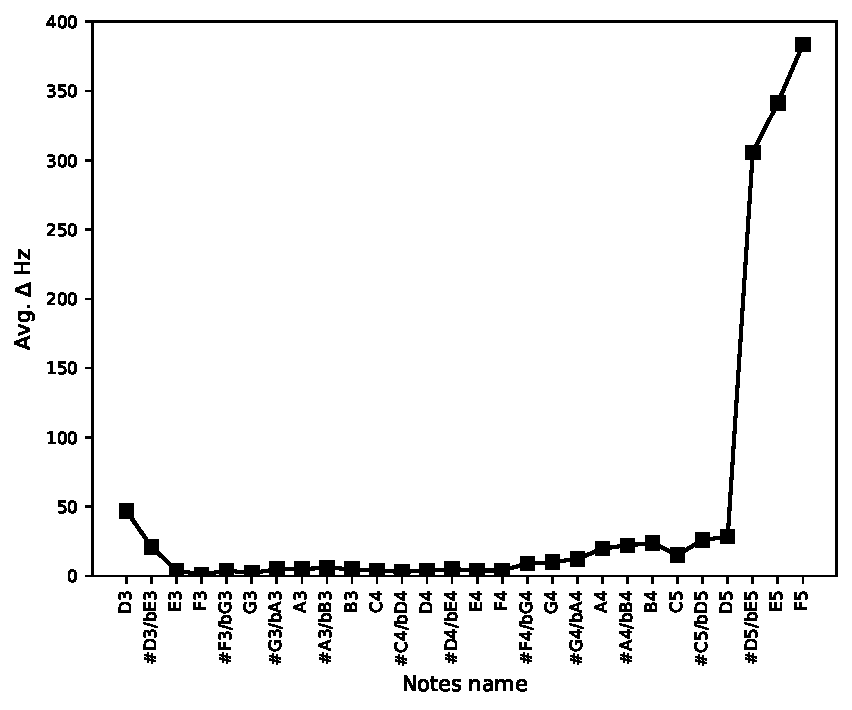
\includegraphics[width=0.99\textwidth]{pitch_range_delta.pdf}
% 	\caption{title}
% 	\label{fig:pitch_range_delta}
% \end{figure}
% \begin{figure}
% 	\includegraphics[width=0.99\textwidth]{figure/svs/pitch_range_mos.pdf}
% 	\caption{title}
% 	\label{fig:pitch_range_mos}
% \end{figure}
图\ref{fig:pitch_range_mos}和图\ref{fig:pitch_range_delta}分别显示了
可以看出,本章提出的模型在PopCS数据集和OpenCpop数据集上进行训练后,在小字组的A,即A3,至小字三组的D,即D5范围内都能有较好的合成质量,但当输入的音高超出此范围后,模型的合成质量就出现显著的下降了。此范围对
\section{本章小结}
本章主要针对翻唱歌声合成提出了一个基于扩散模型和对抗训练的声学模型以合成质量更高的梅尔频谱,由于扩散模型本身推理时间长,本章又实现了\citet{diffsinger}提出的浅扩散机制来优化扩散模型的推理过程。本章提出的基于扩散模型的翻唱歌声合成模型通过参数前端支持适配歌曲的歌词和旋律输入,之后使用声学参数作为条件指导基于扩散模型和对抗训练的歌声合成。在歌声合成数据集上的主要实验结果说明了本章提出的模型和之前的歌声合成声学模型相关工作相比,训练稳定、合成质量更高,在实现了浅扩散机制后在推理速度上也有了极大提升,能适配歌曲翻译的结果,能提供高质量的翻唱合成音频。
